% =====================================================================
%  MAT6202 - Tối ưu hóa nâng cao  |  Bài thuyết trình
%  "Các thuật toán tối ưu hóa hàm tổn thất trong bài toán Hồi quy
%   Logistic" (bộ dữ liệu ứng dụng ngân hàng bán lẻ, ẩn danh).
%
%  Cấu trúc theo `cấu trúc bài thuyết trình mới.txt`;
%  văn phong/mức độ trình bày theo bài mẫu `ref/Nhom03_BaiTap02_v2.pdf`:
%  MỘT Ý / MỘT SLIDE — tiêu đề mục, vài gạch đầu dòng, một hình hoặc một bảng.
%
%  BIÊN DỊCH (tiếng Việt -> cần XeLaTeX):
%     cd presentation_v2
%     xelatex main.tex && biber main && xelatex main.tex && xelatex main.tex
%
%  Mọi CON SỐ trong deck sinh từ code: `python -m optim.diagnostics` (gate.json)
%  rồi `python run_revision.py` (figures + artifacts/rev1_numbers.json).
% =====================================================================
\documentclass[aspectratio=169,11pt]{beamer}

% --- Font & tiếng Việt (XeLaTeX) ---
\usepackage{fontspec}
% Arial/Menlo có sẵn trên macOS. Máy khác: đổi sang DejaVu Serif/Sans/Sans Mono.
\setmainfont{Arial}
\setsansfont{Arial}
\setmonofont{Menlo}

\usepackage{hyperref}
\usepackage{latexsym,amsmath,amssymb,xcolor,multicol,booktabs,array}
\usepackage{graphicx,listings}
\usepackage{siunitx}
\sisetup{group-separator={\,},group-minimum-digits=4,output-decimal-marker={,},
         detect-weight=true,detect-family=true}

\usepackage[backend=biber,style=numeric]{biblatex}
\addbibresource{references.bib}

\graphicspath{{../artifacts/figures/}{images/}}

% --- Metadata ---
\author{Học viên 1 (HV1) \and Học viên 2 (HV2)}   % <-- ĐIỀN TÊN + MSSV thật
\title[Tối ưu trên Hồi quy Logistic]{Các thuật toán tối ưu hóa hàm tổn thất\\ trong bài toán Hồi quy Logistic}
\subtitle{Bộ dữ liệu ứng dụng ngân hàng bán lẻ (ẩn danh)}
\institute{MAT6202 — Tối ưu hóa nâng cao \\ Trường ĐH Khoa học Tự nhiên, ĐHQGHN}
\date{\today}                             % <-- đổi thành ngày thuyết trình

% --- Theme tối giản ---
\usetheme{default}
\usecolortheme{default}
\setbeamertemplate{navigation symbols}{}
\setbeamertemplate{footline}[frame number]

\definecolor{ink}{HTML}{263238}
\definecolor{accent}{HTML}{5B2C82}
\definecolor{accent2}{HTML}{8E6BAF}
\definecolor{warn}{HTML}{C62828}
\definecolor{softgray}{HTML}{F2F0F6}
\definecolor{deepblue}{rgb}{0,0,0.5}
\definecolor{deepred}{rgb}{0.6,0,0}
\definecolor{deepgreen}{rgb}{0,0.5,0}
\definecolor{halfgray}{gray}{0.55}

\setbeamercolor{structure}{fg=accent}
\setbeamercolor{title}{fg=accent}
\setbeamercolor{normal text}{fg=ink}
% Tiêu đề phẳng (không dải màu) cho giống bài mẫu — nhìn "nhẹ" hơn nhiều
\setbeamercolor{frametitle}{fg=accent,bg=}
\setbeamerfont{frametitle}{series=\bfseries,size=\large}
\setbeamercolor{framesubtitle}{fg=accent2}
\setbeamerfont{framesubtitle}{series=\bfseries,size=\footnotesize}
\setbeamercolor{block title}{fg=white,bg=accent}
\setbeamercolor{block body}{bg=softgray}
\setbeamertemplate{itemize items}[circle]
\setbeamertemplate{itemize subitem}[triangle]

% "Nhận xét:" — nhãn phẳng, KHÔNG hộp màu (bài mẫu dùng gạch đầu dòng trơn)
\newcommand{\nx}{\textbf{Nhận xét:}}

% ký hiệu dùng lại
\newcommand{\R}{\mathbb{R}}
\newcommand{\E}{\mathbb{E}}
\newcommand{\wstar}{w^{\star}}
\newcommand{\norm}[1]{\lVert #1 \rVert}
\newcommand{\prox}{\mathrm{prox}}

\lstset{
    basicstyle=\ttfamily\scriptsize,
    keywordstyle=\bfseries\color{deepblue},
    stringstyle=\color{deepgreen},
    commentstyle=\itshape\color{halfgray},
    numbers=left, numberstyle=\tiny\color{halfgray},
    frame=single, rulecolor=\color{accent},
    breaklines=true, showstringspaces=false, language=Python,
}

\definecolor{regimeSafe}{HTML}{31A354}
\definecolor{regimeGray}{HTML}{F16913}
\definecolor{regimeDiv}{HTML}{CB181D}
\begin{document}

% ----------------------------------------------------------- Trang bìa
\begin{frame}[plain]
    \titlepage
\end{frame}

% ----------------------------------------------------------- Nội dung
\begin{frame}{Nội dung trình bày}
  \small
  \begin{center}
  \begin{tabular}{clr}
    \toprule
    STT & Nội dung & Trang\\
    \midrule
    1 & \textbf{Giới thiệu} bài toán, hàm tổn thất và \textbf{tính lồi} & \pageref{sec:1}\\
    2 & \textbf{Lý thuyết} các thuật toán: GD, AGD, Newton, SGD & \pageref{sec:2}\\
    3 & \textbf{Thiết kế} thí nghiệm & \pageref{sec:3}\\
    4 & \textbf{Kết quả}: dò tham số bằng thử và sai & \pageref{sec:4}\\
    5 & Hằng số \textbf{Lipschitz} và chọn bước theo lý thuyết & \pageref{sec:5}\\
    6 & Mở rộng: họ thuật toán \textbf{Ada} và \textbf{Adam} & \pageref{sec:6}\\
    7 & Mở rộng: bài toán \textbf{Lasso} (lồi, không khả vi) & \pageref{sec:7}\\
    8 & \textbf{Kết luận} & \pageref{sec:8}\\
    \bottomrule
  \end{tabular}
  \end{center}
\end{frame}

% =====================================================================
\section{Giới thiệu}
% =====================================================================

\begin{frame}{1. GIỚI THIỆU BÀI TOÁN}{1.1. Phát biểu bài toán}
  \label{sec:1}%
  \small
  \textbf{Bài toán:} dựa trên dữ liệu hành vi của khách hàng trên ứng dụng ngân hàng
  (giao dịch, hoạt động, số dư), dự đoán khách hàng có \textbf{rời bỏ dịch vụ} trong
  3 tháng tiếp theo hay không.
  \vspace{6pt}

  \textbf{Mô hình sử dụng:} biến mục tiêu là biến nhị phân $(0/1)$ nên \textbf{hồi quy logistic}
  là mô hình phù hợp.
  \vspace{6pt}

  \textbf{Trọng tâm của bài:} đối tượng nghiên cứu là \textbf{thuật toán tối ưu}, không phải
  chất lượng dự báo. Nhóm xây dựng hàm tổn thất của hồi quy logistic với các hàm phạt khác nhau:
  \begin{itemize}
    \item Hàm phạt Ridge (trọng tâm — hàm mục tiêu lồi mạnh, khả vi hai lần);
    \item Hàm phạt Lasso (phần mở rộng — lồi nhưng không khả vi).
  \end{itemize}
  \vspace{4pt}
  Mọi so sánh dựa trên \textbf{giá trị hàm mục tiêu} $f(w)$, \textbf{số bước} và \textbf{thời gian}.
\end{frame}

\begin{frame}{1. GIỚI THIỆU BÀI TOÁN}{1.2. Mô hình hồi quy logistic}
  \small
  \textbf{Hàm sigmoid:}
  \[
    \sigma(s)=\frac{1}{1+e^{-s}}\ \in(0,1),\qquad \sigma'(s)=\sigma(s)\big(1-\sigma(s)\big).
  \]
  Với quan sát thứ $i$, đặt $s_i=w^\top x_i$ và $p_i=\sigma(s_i)=\mathbb{P}(y_i{=}1\mid x_i)$.
  \vspace{4pt}

  \textbf{Hàm tổn thất} (ước lượng hợp lý cực đại $\Rightarrow$ log-loss trung bình, kèm hàm phạt):
  \[
    f(w)=-\frac1n\sum_{i=1}^n\Big[y_i\log p_i+(1-y_i)\log(1-p_i)\Big]+r(w)
  \]
  Trong đó:
  \begin{itemize}
    \item $r(w)=0$: trường hợp không có hàm phạt;
    \item $r(w)=\dfrac{\lambda}{2}\norm{w}_2^2$: hàm phạt \textbf{Ridge};
    \item $r(w)=\alpha\norm{w}_1$: hàm phạt \textbf{Lasso}.
  \end{itemize}
\end{frame}

\begin{frame}{1. GIỚI THIỆU BÀI TOÁN}{1.3. Gradient của hàm tổn thất}
  \small
  Xét trường hợp không có hàm phạt. Theo quy tắc đạo hàm hợp:
  \[
    \nabla f(w)=-\frac1n\sum_{i=1}^n\frac{\partial f}{\partial p_i}\frac{\partial p_i}{\partial w}
    =-\frac1n\sum_{i=1}^n\Big(\frac{y_i}{p_i}-\frac{1-y_i}{1-p_i}\Big)\frac{\partial p_i}{\partial w}
    =\frac1n\sum_{i=1}^n\frac{p_i-y_i}{p_i(1-p_i)}\,\frac{\partial p_i}{\partial w}
  \]
  Mặt khác, do $\sigma'(s)=\sigma(s)(1-\sigma(s))$:
  \[
    \frac{\partial p_i}{\partial w}=\sigma'(s_i)\,\frac{\partial s_i}{\partial w}=p_i(1-p_i)\,x_i
    \tag{1}
  \]
  Do đó
  \[
    \boxed{\ \nabla f(w)=\frac1n\sum_{i=1}^n (p_i-y_i)\,x_i=\frac1n X^\top(p-y)\ }
    \tag{2}
  \]
  \nx{} gradient có dạng rất gọn, chi phí tính là $O(nd)$ — một phép nhân ma trận--vector.
\end{frame}

\begin{frame}{1. GIỚI THIỆU BÀI TOÁN}{1.4. Ma trận Hessian và chứng minh tính lồi}
  \small
  Từ (1) và (2), đạo hàm tiếp theo $w$:
  \[
    \nabla^2 f(w)=\frac1n\sum_{i=1}^n p_i(1-p_i)\,x_i x_i^\top=\frac1n X^\top S X,
    \qquad S=\mathrm{diag}\big(p_i(1-p_i)\big).
  \]
  Với mọi vector $v\in\R^d$:
  \[
    v^\top \nabla^2f(w)\, v=\frac1n\sum_{i=1}^n \underbrace{p_i(1-p_i)}_{>0}\,\big(x_i^\top v\big)^2\ \ge\ 0 .
  \]
  \begin{itemize}
    \item Hessian \textbf{nửa xác định dương} $\Rightarrow$ $f$ là \textbf{hàm lồi} $\Rightarrow$
          mọi điểm dừng đều là cực tiểu toàn cục: chỉ cần tìm điểm thỏa $\nabla f(w)=0$.
    \item Hàm tổn thất \textbf{không có nghiệm đóng} $\Rightarrow$ bắt buộc giải bằng phương pháp lặp.
  \end{itemize}
  \vspace{2pt}
  \textit{Lưu ý: gradient và Hessian của hàm phạt Ridge được cộng thêm trực tiếp:}
  $\nabla r(w)=\lambda w$, $\nabla^2 r(w)=\lambda I$.
\end{frame}

% =====================================================================
\section{Lý thuyết các thuật toán}
% =====================================================================

\begin{frame}{2. LÝ THUYẾT CÁC THUẬT TOÁN}{2.1. Bốn thuật toán được thử nghiệm}
  \label{sec:2}%
  \small
  \begin{center}
  \begin{tabular}{lccc}
    \toprule
    Thuật toán & Công thức cập nhật & Tốc độ hội tụ & Chi phí/bước\\
    \midrule
    Gradient Descent & $w^+=w-t\,\nabla f(w)$ & tuyến tính $\big(1-\tfrac1\kappa\big)^k$ & $O(nd)$\\
    Accelerated GD & thêm động lượng & tuyến tính $\big(1-\tfrac{1}{\sqrt\kappa}\big)^k$ & $O(nd)$\\
    Newton & $w^+=w-t\,\big(\nabla^2f\big)^{-1}\nabla f$ & \textbf{bậc hai} (cục bộ) & $O(nd^2{+}d^3)$\\
    SGD / Mini-batch & gradient trên tập con & dưới tuyến tính $O(1/k)$ & $O(bd)$\\
    \bottomrule
  \end{tabular}
  \end{center}
  \vspace{6pt}
  \nx{}
  \begin{itemize}
    \item Cả bốn cùng giải một hàm mục tiêu, chỉ khác \textbf{lượng thông tin} dùng ở mỗi bước:
          GD/AGD dùng gradient, Newton dùng thêm Hessian, SGD dùng ước lượng của gradient.
    \item Số bước ít hơn \emph{không} đồng nghĩa với nhanh hơn: phải nhân với chi phí mỗi bước
          $\Rightarrow$ mọi so sánh trong bài đều vẽ theo \textbf{cả số bước và thời gian}.
  \end{itemize}
\end{frame}

\begin{frame}{2. LÝ THUYẾT CÁC THUẬT TOÁN}{2.2. Gradient Descent và ba cách chọn độ dài bước}
  \small
  Chọn điểm tiếp theo theo công thức $\ w^{+}=w-t\,\nabla f(w)$.
  \vspace{4pt}
  \begin{itemize}
    \item \textbf{Độ dài bước cố định:} giá trị $t$ không đổi qua các lần lặp. Điều kiện hội tụ:
          $t<\dfrac{2}{L}$, giá trị tốt nhất theo lý thuyết là $t=\dfrac1L$.
    \item \textbf{Backtracking (Armijo):} mỗi lần lặp bắt đầu với $t=t_{init}$, và trong khi
          \[
            f\big(w-t\nabla f(w)\big)>f(w)-c\,t\,\norm{\nabla f(w)}_2^2
          \]
          thì cập nhật $t=\rho\,t$ (với $0<\rho<1$, $0<c<\tfrac12$); ngược lại thực hiện bước GD.
    \item \textbf{Acceleration (Nesterov):} chọn $w^{(0)}=w^{(-1)}$, lặp
          \[
            v=w^{(k-1)}+\beta\big(w^{(k-1)}-w^{(k-2)}\big),\qquad
            w^{(k)}=v-t\,\nabla f(v)
          \]
          với $\beta=\dfrac{\sqrt\kappa-1}{\sqrt\kappa+1}$ cho hàm \textbf{lồi mạnh}
          (dạng $\frac{\sqrt L-\sqrt\mu}{\sqrt L+\sqrt\mu}$ trong~\cite{nesterov2018lectures},
          chia cho $\sqrt\mu$ thì ra dạng trên), hoặc $\beta_k=\tfrac{k-2}{k+1}$ cho hàm
          \textbf{lồi thường}~\cite{beck2009fista} --- lược đồ thứ hai không chứa hằng số nào của
          bài toán, nên $t$ ở đó là tham số tự do (mục 4.11).
  \end{itemize}
\end{frame}

\begin{frame}{2. LÝ THUYẾT CÁC THUẬT TOÁN}{2.3. Vì sao Acceleration nhanh hơn: $\kappa$ so với $\sqrt\kappa$}
  \small
  Với hàm lồi mạnh, số bước cần thiết để đạt sai số $\epsilon$:
  \begin{center}
  \begin{tabular}{lcc}
    \toprule
    & Tốc độ hội tụ & Số bước cần\\
    \midrule
    Gradient Descent & $f(w_k)-f^\star\le\big(1-\tfrac{1}{\kappa}\big)^k\big(f(w_0)-f^\star\big)$
                     & $O\big(\kappa\log\tfrac1\epsilon\big)$\\
    Accelerated GD   & $f(w_k)-f^\star\le\big(1-\tfrac{1}{\sqrt\kappa}\big)^k\,L\norm{w_0-\wstar}^2$
                     & $O\big(\sqrt\kappa\log\tfrac1\epsilon\big)$\\
    \bottomrule
  \end{tabular}
  \end{center}
  \vspace{6pt}
  \nx{}
  \begin{itemize}
    \item Hai thuật toán có \textbf{cùng chi phí mỗi bước} $O(nd)$ (một lần tính gradient), nhưng
          AGD đổi $\kappa$ thành $\sqrt\kappa$ trong tốc độ.
    \item Với $\kappa=\num{14069}$ của bộ dữ liệu này (mục 3.3): $\kappa$ so với
          $\sqrt\kappa\approx119$ — chênh lệch \textbf{hơn hai bậc} về số bước. Mục 5.5 kiểm
          chứng bằng thực nghiệm: tỉ số độ dốc log--log đo được là $1{,}98\approx2$.
    \item Đánh đổi: quỹ đạo của AGD \textbf{không đơn điệu} (có dao động nhẹ khi gần nghiệm).
  \end{itemize}
\end{frame}

\begin{frame}{2. LÝ THUYẾT CÁC THUẬT TOÁN}{2.4. Thuật toán Newton}
  \small
  \begin{itemize}
    \item \textbf{Pure Newton:} $\ w^{(k)}=w^{(k-1)}-\big(\nabla^2f(w^{(k-1)})\big)^{-1}\nabla f(w^{(k-1)})$.
    \item \textbf{Damped Newton — độ dài bước cố định:} $\ w^{+}=w-t\big(\nabla^2f(w)\big)^{-1}\nabla f(w)$.
    \item \textbf{Damped Newton — Backtracking:} với hướng $v=-\big(\nabla^2f(w)\big)^{-1}\nabla f(w)$,
          bắt đầu $t=t_{init}$ và trong khi $f(w+tv)>f(w)+c\,t\,\nabla f(w)^\top v$ thì $t=\rho t$.
  \end{itemize}
  \vspace{6pt}
  \textbf{Lưu ý quan trọng khi cài đặt:} không đi tìm ma trận nghịch đảo của Hessian.
  Thay vào đó, tìm nghiệm của hệ phương trình
  \[
    \nabla^2 f(w)\, v=-\nabla f(w)
  \]
  bằng khử Gauss (phân tích LU), Conjugate Gradient hoặc phân tích Cholesky. Đây cũng chính là
  ý tưởng của hai solver \texttt{newton-cg} và \texttt{newton-cholesky} trong \texttt{scikit-learn}.
  \vspace{4pt}

  \nx{} Newton trên hàm log-loss chính là thuật toán \textbf{IRLS} quen thuộc trong lý thuyết
  mô hình tuyến tính tổng quát (GLM)~\cite{nocedal2006numerical}.
\end{frame}

\begin{frame}{2. LÝ THUYẾT CÁC THUẬT TOÁN}{2.5. Newton: hội tụ bậc hai cục bộ và định lý Kantorovich}
  \small
  Thuật toán Newton có \textbf{hai pha} rõ rệt~\cite{boyd2004convex}:
  \begin{itemize}
    \item \textbf{Pha damped} (khi còn ở xa nghiệm): mỗi bước làm giảm $f$ ít nhất một lượng
          hằng số $\gamma>0$ $\Rightarrow$ số bước của pha này bị chặn bởi $\big(f(w_0)-f^\star\big)/\gamma$.
    \item \textbf{Pha hội tụ bậc hai} (khi đã đủ gần nghiệm): độ dài bước $t=1$ luôn được chấp nhận và
          \[
            \norm{w_{k+1}-\wstar}\ \le\ c\,\norm{w_k-\wstar}^2
          \]
          nghĩa là \textbf{số chữ số đúng tăng gấp đôi} sau mỗi bước.
  \end{itemize}
  \vspace{4pt}
  \textbf{Định lý Kantorovich} (điều kiện đủ để Newton thuần hội tụ ngay từ $w_0$): nếu
  $\norm{\nabla^2f(w_0)^{-1}}\le\beta_0$, $\norm{\nabla^2f(w_0)^{-1}\nabla f(w_0)}\le\eta_0$,
  Hessian Lipschitz với hằng số $M$, và
  \[
    h_0=\beta_0\,M\,\eta_0\ \le\ \tfrac12
  \]
  thì dãy lặp Newton hội tụ về $\wstar$ với tốc độ bậc hai.
  \vspace{2pt}

  \nx{} $h_0\le\frac12$ chính là \textbf{bán kính hội tụ}: khởi tạo ngoài vùng này, Newton thuần
  có thể vọt lố — đó là lý do cần damping / backtracking.
\end{frame}

\begin{frame}{2. LÝ THUYẾT CÁC THUẬT TOÁN}{2.6. Stochastic Gradient Descent (SGD)}
  \small
  Chọn ngẫu nhiên tập con $I_k\subseteq\{1,\dots,n\}$ với $|I_k|=b\ll n$, lặp lại
  \[
    w^{(k)}=w^{(k-1)}-t_k\cdot\frac1b\sum_{i\in I_k}\nabla f_i\big(w^{(k-1)}\big).
  \]
  \begin{itemize}
    \item Trung bình gradient trên mini-batch là \textbf{ước lượng không chệch} của gradient toàn bộ dữ liệu;
          $b=1$ là SGD, $b>1$ là mini-batch.
    \item Phương sai của ước lượng tỉ lệ $\sigma^2/b$ — đây là nguồn gốc của mọi hiện tượng ở phần 4.
  \end{itemize}
  \vspace{4pt}
  Hai cách chọn độ dài bước:
  \begin{itemize}
    \item \textbf{Bước cố định:} hội tụ nhanh lúc đầu nhưng dừng lại ở một \textbf{sàn phương sai}
          $\ \limsup_k \E\big[f(w_k)-f^\star\big]\ \le\ \dfrac{t\,L\,\sigma^2}{2\mu\,b}$ — tỉ lệ với $t/b$.
    \item \textbf{Bước giảm dần} (Robbins--Monro~\cite{robbins1951stochastic}): $\sum_k t_k=\infty$,
          $\sum_k t_k^2<\infty$ (ví dụ $t_k=t_0/k$ hoặc $t_0/\sqrt k$) $\Rightarrow$ hội tụ thật, tốc độ $O(1/k)$.
  \end{itemize}
\end{frame}

\begin{frame}{2. LÝ THUYẾT CÁC THUẬT TOÁN}{2.7. Bất biến affine: vì sao phải chuẩn hóa dữ liệu}
  \small
  Đổi biến khả nghịch $w=A\,v$ và đặt $g(v)=f(Av)$. Khi đó
  $\nabla g(v)=A^\top\nabla f$, $\nabla^2 g(v)=A^\top\big(\nabla^2 f\big)A$.
  \begin{columns}[T]
    \begin{column}{0.5\textwidth}
      \textbf{Newton — bất biến affine:}
      \[
        \Delta_v=-\big(A^\top H A\big)^{-1}A^\top\nabla f=A^{-1}\Delta_w
      \]
      Quỹ đạo Newton trên hai hệ tọa độ là \emph{một} quỹ đạo
      $\Rightarrow$ số bước \textbf{không đổi} khi đổi thang đo các biến.
    \end{column}
    \begin{column}{0.5\textwidth}
      \textbf{Gradient Descent — không bất biến:}
      \[
        \Delta_v=-t\,A^\top\nabla f\ \ne\ A^{-1}\Delta_w
      \]
      Bước GD phụ thuộc hoàn toàn vào đơn vị đo của từng cột
      $\Rightarrow$ thang đo lệch làm $\kappa$ nổ và GD chậm đi rất nhiều.
    \end{column}
  \end{columns}
  \vspace{6pt}
  {\footnotesize\nx{}}
  \begin{itemize}\scriptsize
    \item Đây là lý do \textbf{bắt buộc chuẩn hóa} $X$: bản chất là ta \emph{làm giúp} GD phép đổi
          biến mà Newton tự làm được.
    \item Kiểm chứng ở $\lambda=0$ (log-loss thuần, bất biến affine \emph{thật sự}): Newton dùng
          \textbf{đúng 17 bước} trên cả bộ chuẩn hóa lẫn bộ thô --- hai bài toán lệch nhau 19 bậc
          độ lớn về thang đo. Ở $d=415$ bản thân $\kappa$ \emph{không đo được} (Hessian tại $\wstar$
          của bộ thô có 11 trị riêng không dương), nên bằng chứng nằm ở \textbf{số bước bằng nhau},
          không phải ở giá trị $\kappa$.
    \item Với hàm phạt Ridge, số hạng $\tfrac\lambda2\norm{w}^2$ \emph{phá vỡ} bất biến affine
          nên Newton không còn miễn nhiễm hoàn toàn (mục 4.1).
  \end{itemize}
\end{frame}

\begin{frame}{2. LÝ THUYẾT CÁC THUẬT TOÁN}{2.8. Newton yêu cầu ma trận đủ hạng}
  \small
  Thuật toán Newton phải giải hệ $\Big(\dfrac1n X^\top S X+\lambda I\Big)v=-\nabla f(w)$.
  \begin{itemize}
    \item Nếu $X$ \textbf{không đủ hạng} thì $X^\top S X$ suy biến: khi $\lambda\to0$ hệ vô định,
          Cholesky thất bại; khi $\lambda>0$ hệ vẫn giải được nhưng $\kappa$ rất lớn, nghiệm mất chính xác.
    \item GD/AGD \emph{không báo lỗi} trong trường hợp này — chúng vẫn chạy, chỉ là nghiệm không duy nhất.
          Sai lầm im lặng nguy hiểm hơn sai lầm ồn ào.
  \end{itemize}
  \vspace{6pt}
  \textbf{Ba nguồn suy biến thường gặp và cách xử lý:}
  \begin{center}
  \begin{tabular}{ll}
    \toprule
    Nguồn suy biến & Cách xử lý\\
    \midrule
    One-hot giữ đủ $k$ mức $+$ hệ số chặn & mã hóa với \texttt{drop\_first=True}\\
    Biến đa thức sinh từ biến 0/1 ($b^2=b$) & chỉ mở rộng đa thức trên các biến liên tục\\
    Đa cộng tuyến gần đúng (VIF cao) & cắt tỉa theo tương quan và VIF\\
    \bottomrule
  \end{tabular}
  \end{center}
  \vspace{4pt}
  \nx{} hai yêu cầu \emph{chuẩn hóa} và \emph{đủ hạng} quyết định toàn bộ khâu xử lý dữ liệu ở phần 3.
\end{frame}

% =====================================================================
\section{Thiết kế thí nghiệm}
% =====================================================================

\begin{frame}{3. THIẾT KẾ THÍ NGHIỆM}{3.1. Bộ dữ liệu}
  \label{sec:3}%
  \footnotesize
  \textbf{Nguồn:} dữ liệu ứng dụng ngân hàng bán lẻ (ẩn danh), gồm 6 bảng nối theo mã khách hàng.
  \begin{center}\footnotesize
  \begin{tabular}{lll}
    \toprule
    Bảng & Quy mô & Nội dung\\
    \midrule
    Khách hàng      & $\sim$290 nghìn dòng & thông tin nhân khẩu học (tĩnh)\\
    Giao dịch       & $\sim$1{,}4 triệu dòng & số lần / giá trị / loại giao dịch\\
    Hoạt động       & $\sim$16 triệu dòng & thao tác phi tài chính trên ứng dụng\\
    Tiền gửi / Tín dụng / Thẻ & $\sim$1{,}3 triệu dòng & số dư theo tháng\\
    \bottomrule
  \end{tabular}
  \end{center}
  \vspace{6pt}
  \textbf{Cách gán nhãn (tránh rò rỉ thông tin):} chọn mốc $T$, hai cửa sổ tách rời, đều
  \emph{nửa mở bên trái} để không ngày nào bị đếm hai lần:
  \begin{itemize}
    \item cửa sổ quan sát $(T-3\text{ tháng},\,T]$: \emph{chỉ} dùng để sinh đặc trưng;
    \item cửa sổ kết quả $(T,\,T+3\text{ tháng}]$: \emph{chỉ} dùng để sinh nhãn $y$.
  \end{itemize}
  $y_i=1$ nếu khách hàng không phát sinh giao dịch \emph{và} không có hoạt động nào trong cửa sổ kết quả.
  \vspace{2pt}

  \textbf{Xếp chồng ba mốc.} Với $K=H=3$ tháng, ba cặp cửa sổ lát kín năm 2019:
  $T\in\{$03-31, 06-30, 09-30$\}$. Mỗi dòng của $X$ là một cặp \textbf{(khách hàng, mốc)}.
  \vspace{2pt}

  \textbf{Kết quả:} $n=\num{75026}$ dòng, tỉ lệ rời bỏ $10{,}8\%$ — toàn bộ dùng cho thí nghiệm tối ưu.
\end{frame}

\begin{frame}{3. THIẾT KẾ THÍ NGHIỆM}{3.2. Xây dựng ma trận thiết kế $X$}
  \footnotesize
  Bảy bước xử lý, theo đúng thứ tự:
  \begin{center}\scriptsize
  \begin{tabular}{clp{6.6cm}}
    \toprule
    Bước & Nội dung & Lý do\\
    \midrule
    1 & Gộp về 1 dòng / khách hàng & dữ liệu gốc là dạng bảng nhiều dòng theo tháng\\
    2 & Điền khuyết $+$ \texttt{log1p} & không được sót NaN; giảm đuôi dày của biến tiền tệ\\
    3 & One-hot \texttt{drop\_first} & \textbf{bắt buộc}: tránh cộng tuyến hoàn hảo (mục 2.8)\\
    4 & Chuẩn hóa $z$-score & \textbf{bắt buộc} với thuật toán bậc nhất (mục 2.7)\\
    5 & Cắt tỉa tương quan $+$ VIF & giảm cộng tuyến \emph{gần đúng}, hạ số điều kiện\\
    6 & QR có xoay cột & \textbf{bắt buộc}: hai bước trên không bắt được cộng tuyến \emph{chính xác}\\
    7 & (tùy chọn) đặc trưng đa thức & chỉ trên biến liên tục, để không sinh cột trùng\\
    \bottomrule
  \end{tabular}
  \end{center}
  \vspace{4pt}
  \nx{} \textbf{không chia train/test}. Đây là bài toán tối ưu: hàm mục tiêu $f(w)$ được xác định
  trên \emph{bất kỳ} cặp $(X,y)$ nào, và mọi đại lượng ta so sánh ($L$, $\mu$, $\kappa$, số bước,
  thời gian, $f-f^\star$) đều không cần tập kiểm tra. Chia chỉ làm mất 25\% dữ liệu.
  Bốn bước 3--6 đều xuất phát từ yêu cầu của \emph{thuật toán}, không phải của mô hình.
\end{frame}

\begin{frame}{3. THIẾT KẾ THÍ NGHIỆM}{3.3. Các bộ dữ liệu dùng trong thí nghiệm}
  \small
  \begin{center}
  \begin{tabular}{lcccl}
    \toprule
    Bộ dữ liệu & $d$ & Hạng & $\kappa$ ($\lambda{=}10^{-3}$) & Dùng cho\\
    \midrule
    \texttt{ridge}      & 415 & 415 (đủ)  & \num{14070}   & thí nghiệm chính (GD/AGD/Newton/SGD)\\
    \texttt{ridge\_raw} & 415 & 376       & \num{2.66e19} & đối chứng: \emph{không} chuẩn hóa\\
    \texttt{lasso}      & 519 & 506       & \num{19700}   & phần mở rộng L1 (giữ biến dư thừa)\\
    \bottomrule
  \end{tabular}
  \end{center}
  \vspace{4pt}
  {\footnotesize\nx{}}
  \begin{itemize}\footnotesize
    \item \texttt{ridge} và \texttt{ridge\_raw} có \textbf{đúng cùng các cột}, chỉ khác đơn vị đo
          $\Rightarrow$ so sánh hai bộ này cô lập được đúng tác động của chuẩn hóa.
    \item Chỉ \texttt{ridge} \textbf{đủ hạng} $\Rightarrow$ chỉ nó chạy được Newton. Đủ hạng không
          tự nhiên mà có: sau lọc tương quan và VIF vẫn sót cộng tuyến \emph{chính xác}, phải thêm
          bước \textbf{QR có xoay cột} mới bảo đảm (mục 2.8).
    \item \texttt{ridge\_raw} hạng 376/415 không phải vì thiếu cột, mà vì $\kappa\approx10^{19}$
          \emph{vượt} dải biểu diễn của số thực 64 bit: $\lambda I$ thành vô hình, Hessian suy biến
          về mặt số học.
    \item \texttt{lasso} cố ý \emph{không} cắt hết biến dư thừa, để hàm phạt L1 có việc để làm.
  \end{itemize}
\end{frame}

\begin{frame}{3. THIẾT KẾ THÍ NGHIỆM}{3.4. Các thí nghiệm và tiêu chí so sánh}
  \small
  \begin{block}{Danh sách thí nghiệm}
    \footnotesize
    \begin{itemize}
      \item \textbf{So sánh dữ liệu chuẩn hóa và không chuẩn hóa} — GD, AGD, Newton trên
            \texttt{ridge} và \texttt{ridge\_raw}.
      \item \textbf{Thử nghiệm siêu tham số của từng thuật toán} — GD: quét độ dài bước cố định,
            quét $(c,\rho)$ của backtracking; Newton: pure / damped cố định / damped backtracking;
            SGD: quét kích thước mini-batch và lịch giảm bước.
      \item \textbf{So sánh các thuật toán} với siêu tham số tốt nhất tìm được, trên cùng
            bộ dữ liệu chuẩn hóa.
      \item \textbf{Đối chiếu với \texttt{scikit-learn}} (\texttt{lbfgs}, \texttt{newton-cholesky}, \texttt{saga}).
    \end{itemize}
  \end{block}
  \textbf{Điều kiện giữ cố định:} cùng điểm khởi tạo $w_0=0$; cùng $\lambda=10^{-3}$;
  cùng tiêu chí dừng $\norm{\nabla f(w)}_2<\varepsilon$; cùng giá trị tham chiếu $f^\star$
  (chạy Newton tới $\norm{\nabla f}_2<10^{-14}$, mục 4.2).
  \vspace{2pt}

  \textbf{Ba chỉ số báo cáo:} $f(w)-f^\star$ (trục tung, thang $\log$), \textbf{số bước}, \textbf{thời gian}.
\end{frame}

% =====================================================================
\section{Kết quả: dò tham số bằng thử và sai}
% =====================================================================

\begin{frame}{4. KẾT QUẢ: DÒ THAM SỐ BẰNG THỬ VÀ SAI}{4.1. Dữ liệu chuẩn hóa và không chuẩn hóa}
  \label{sec:4}%
  \begin{center}
    \IfFileExists{../artifacts/figures/standardization_contrast.png}
      {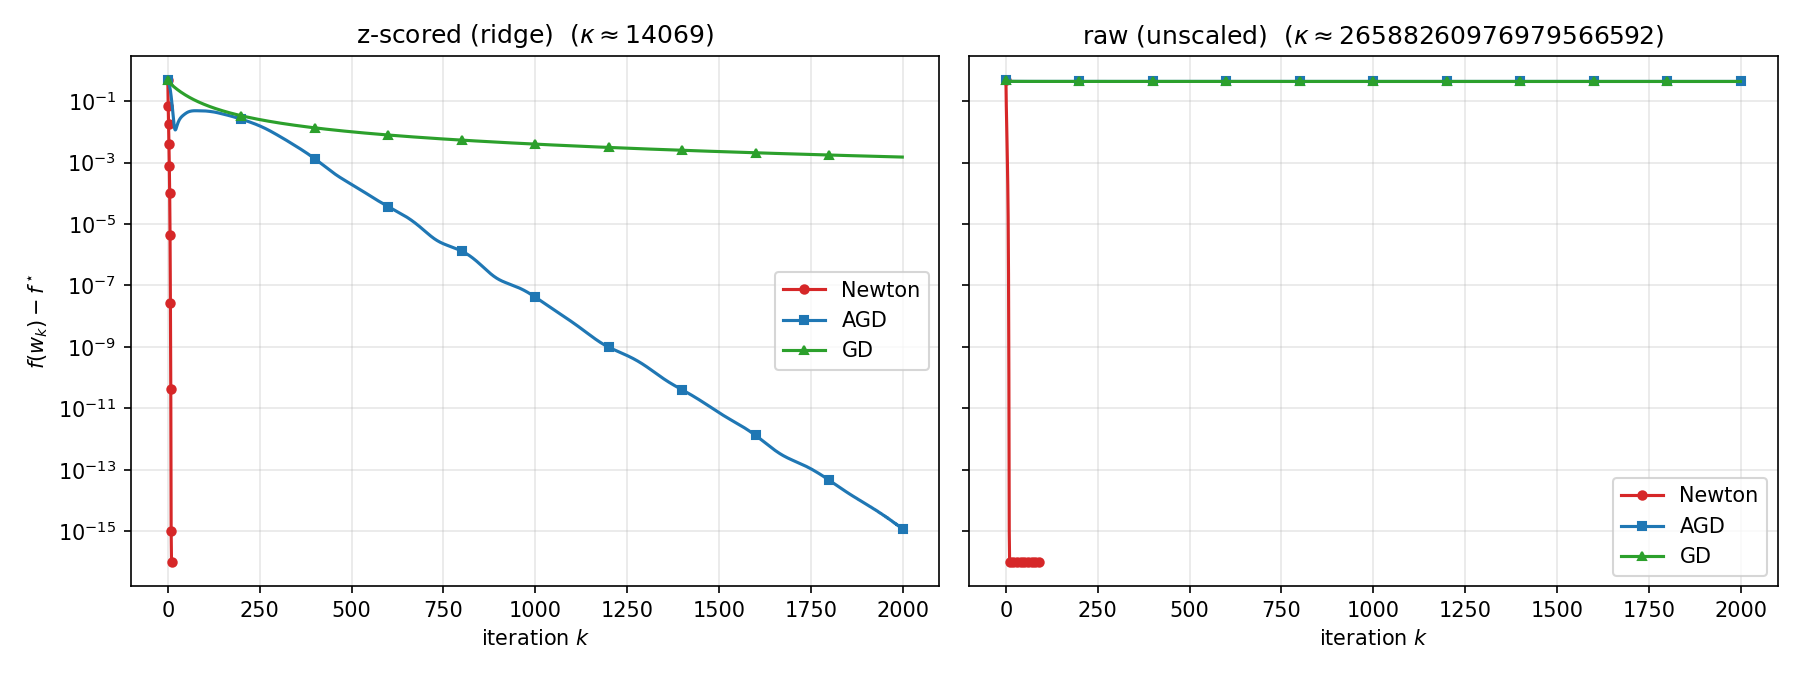
\includegraphics[width=0.90\linewidth]{standardization_contrast}}
      {\footnotesize\textit{[standardization\_contrast.png]}}
  \end{center}
  \vspace{-2pt}
  {\scriptsize\nx{} \textbf{không chuẩn hóa} thì GD và AGD gần như \emph{không giảm được gì} --- sau
  \num{2000} bước còn cách nghiệm \textbf{0{,}434}, trong khi bộ chuẩn hóa cho AGD
  $1{,}2\times10^{-15}$ và GD $1{,}5\times10^{-3}$ ($\kappa$: \num{1.4e4} so với \num{2.7e19},
  \textbf{15 bậc độ lớn}). Ở $d=415$ Newton \textbf{không còn chạy được} chứ không phải chỉ chậm:
  $\lambda I$ chìm dưới sai số làm tròn nên Hessian suy biến về mặt số học (hạng \num{376}/\num{415}),
  chạm trần \num{100} bước so với \textbf{11} bước trên bộ chuẩn hóa. Vì vậy chuẩn hóa là
  \textbf{ràng buộc bắt buộc}, không phải mẹo tinh chỉnh.}
\end{frame}

\begin{frame}{4. KẾT QUẢ: DÒ THAM SỐ BẰNG THỬ VÀ SAI}{4.2. Xác định $f^\star$ --- mốc tham chiếu cho mọi hình phía sau}
  \scriptsize
  Mọi hình trong bài vẽ $\log\big(f(w_k)-f^\star\big)$, nên $f^\star$ phải được xác định
  \textbf{trước}, một lần, và phải \emph{chứng nhận được}. Cách làm:
  \begin{itemize}\scriptsize\itemsep=1pt
    \item Chạy \textbf{damped Newton tới $\norm{\nabla f}<10^{-14}$} (backtracking mặc định
          $t_0=1$, $\rho=0{,}5$, $c=10^{-4}$; 15 vòng, \num{10.4}s), rồi lấy giá trị tại
          \textbf{iterate CUỐI CÙNG}:
          \[ f^\star=\mathbf{0{,}212258252065506},\qquad \norm{\nabla f(w^\star)}=\num{7.9e-15}. \]
    \item \textbf{Chứng chỉ.} Với $f$ lồi mạnh hệ số $\mu$ trên tập mức, bất đẳng thức PL cho
          \[ 0\ \le\ f^\star-f_{\text{true}}^\star\ \le\ \frac{\norm{\nabla f(w^\star)}^2}{2\mu^\star}
             \ =\ \num{3.1e-26}, \]
          với $\mu^\star=\lambda_{\min}\big(\nabla^2f(w^\star)\big)=\num{1.001e-3}$ \emph{đo được},
          không phải $\lambda$: hệ số chặn không bị phạt nên $\lambda I\preceq\nabla^2f$ chỉ đúng
          trên các tọa độ bị phạt (mục 5.1). Sai số này nhỏ hơn sàn $10^{-16}$ của mọi hình
          \textbf{10 bậc}, nên $f^\star$ coi như chính xác tuyệt đối.
    \item \textbf{Không lấy $\min$ của lịch sử.} $\min_k f(w_k)$ báo cáo một điểm \emph{khác} với
          điểm thuật toán trả về, và nó bào mòn khoảng cách của mọi phương pháp khác theo hướng
          có lợi cho ta --- đọc lên là thiên vị.
    \item \textbf{Kiểm chứng độc lập}: \texttt{sklearn lbfgs} trên cùng hàm mục tiêu dừng ở
          $f^\star+\num{2.2e-13}$ (mục 4.19) --- hai cài đặt hoàn toàn khác nhau gặp nhau ở chữ số
          thứ 13.
  \end{itemize}
  \vspace{1pt}
  {\scriptsize\nx{} lần chạy này \emph{chỉ} để lấy $f^\star$ --- nó dùng tham số mặc định của thư
  viện nên \textbf{không} xuất hiện như một đường trong mục 4.17--4.18; bảy đường ở đó đều là
  cấu hình dò tay. \texttt{optim/reference.py}}
\end{frame}

\begin{frame}{4. KẾT QUẢ: DÒ THAM SỐ BẰNG THỬ VÀ SAI}{4.3. Newton --- dò bước cố định}
  \begin{center}
    {\large\color{accent}\textbf{$\rightarrow$ Chọn $t = 1$ (pure Newton)}}
  \end{center}
  \vspace{-6pt}
  \begin{center}
    \IfFileExists{../artifacts/figures/tune_newton_fixed.png}
      {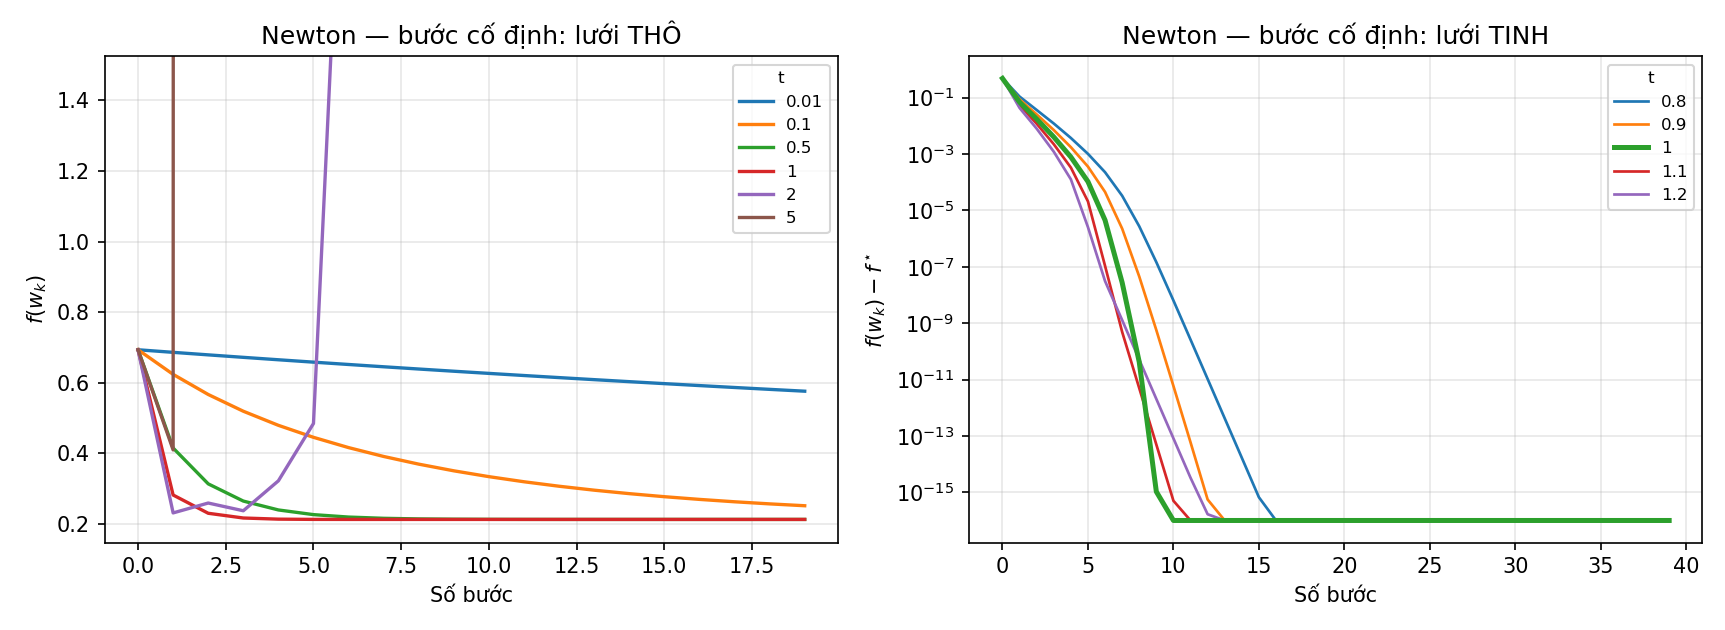
\includegraphics[width=0.70\linewidth]{tune_newton_fixed}}{}
  \end{center}
  \vspace{-2pt}
  {\scriptsize\nx{} quy trình dùng chung cho \emph{mọi} thuật toán trong mục này: một
  \textbf{lưới thô} $[0{,}01;\,0{,}1;\,0{,}5;\,1;\,2;\,5]$ chạy 20 vòng, rồi một \textbf{lưới tinh}
  quanh vùng thắng, rồi \emph{nhìn hình} mà chọn --- không có hàm chấm điểm nào.
  Lưới thô hiện đủ \textbf{ba chế độ}: $t\le0{,}1$ bò chậm ($3{,}6\times10^{-1}$;
  $3{,}9\times10^{-2}$), $t=0{,}5$--$1$ về tới độ chính xác máy ($2{,}8\times10^{-17}$), còn
  $t=2$ và $t=5$ \textbf{chết thật} --- dừng ở vòng 15 và vòng 5 vì $\norm{w}$ vọt đi, $S$ chạm
  đáy và Cholesky hỏng (xem mục 4.6). Lưới tinh thì \textbf{không phân biệt được gì}: mọi
  $t\in[0{,}8;\,1{,}2]$ đều tới độ chính xác máy nên $f-f^\star$ cuối giống hệt nhau; phải đổi tiêu
  chí sang \textbf{số vòng}, khi đó $t=1$ thắng.}
\end{frame}

\begin{frame}{4. KẾT QUẢ: DÒ THAM SỐ BẰNG THỬ VÀ SAI}{4.4. Newton --- dò $(\rho, c)$ của backtracking}
  \begin{center}
    \IfFileExists{../artifacts/figures/tune_newton_bt_grid.png}
      {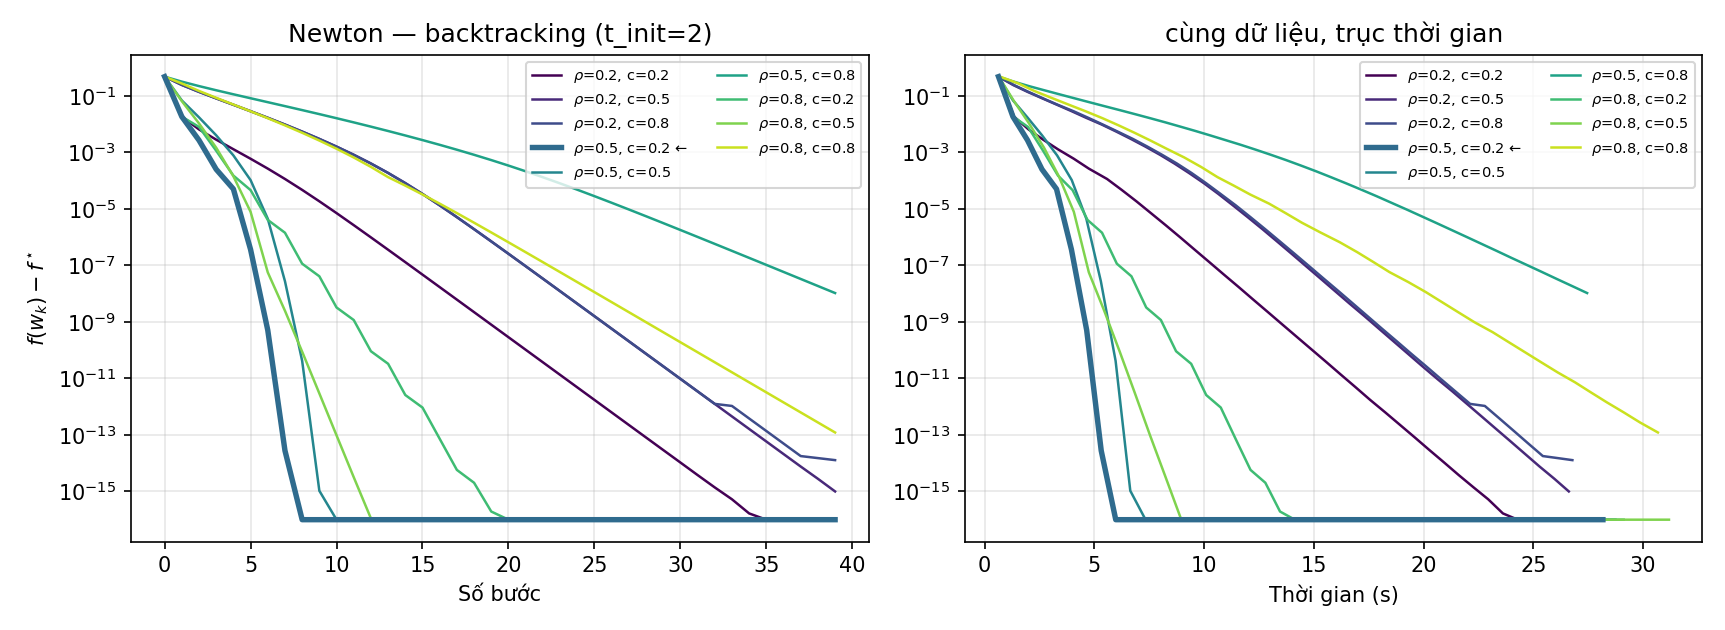
\includegraphics[width=0.94\linewidth]{tune_newton_bt_grid}}{}
  \end{center}
  \vspace{-2pt}
  {\scriptsize\nx{}}
  \begin{itemize}\scriptsize\itemsep=1pt
    \item $\rho=\mathbf{0{,}5}$, $c=\mathbf{0{,}2}$ thắng \emph{cả hai} trục ($\sim$8 vòng,
          $\num{5.5}$s) --- khác hẳn GD ở mục 4.8, nơi hai trục cho hai câu trả lời khác nhau.
    \item $c$ nhỏ $=$ điều kiện Armijo dễ thỏa $=$ giữ được bước gần $1$, tức gần pure Newton ---
          đúng thứ ta muốn khi đã ở gần nghiệm.
  \end{itemize}
\end{frame}

\begin{frame}{4. KẾT QUẢ: DÒ THAM SỐ BẰNG THỬ VÀ SAI}{4.5. Newton --- so sánh ba cách chọn bước}
  \begin{center}
    \IfFileExists{../artifacts/figures/tune_cmp_newton.png}
      {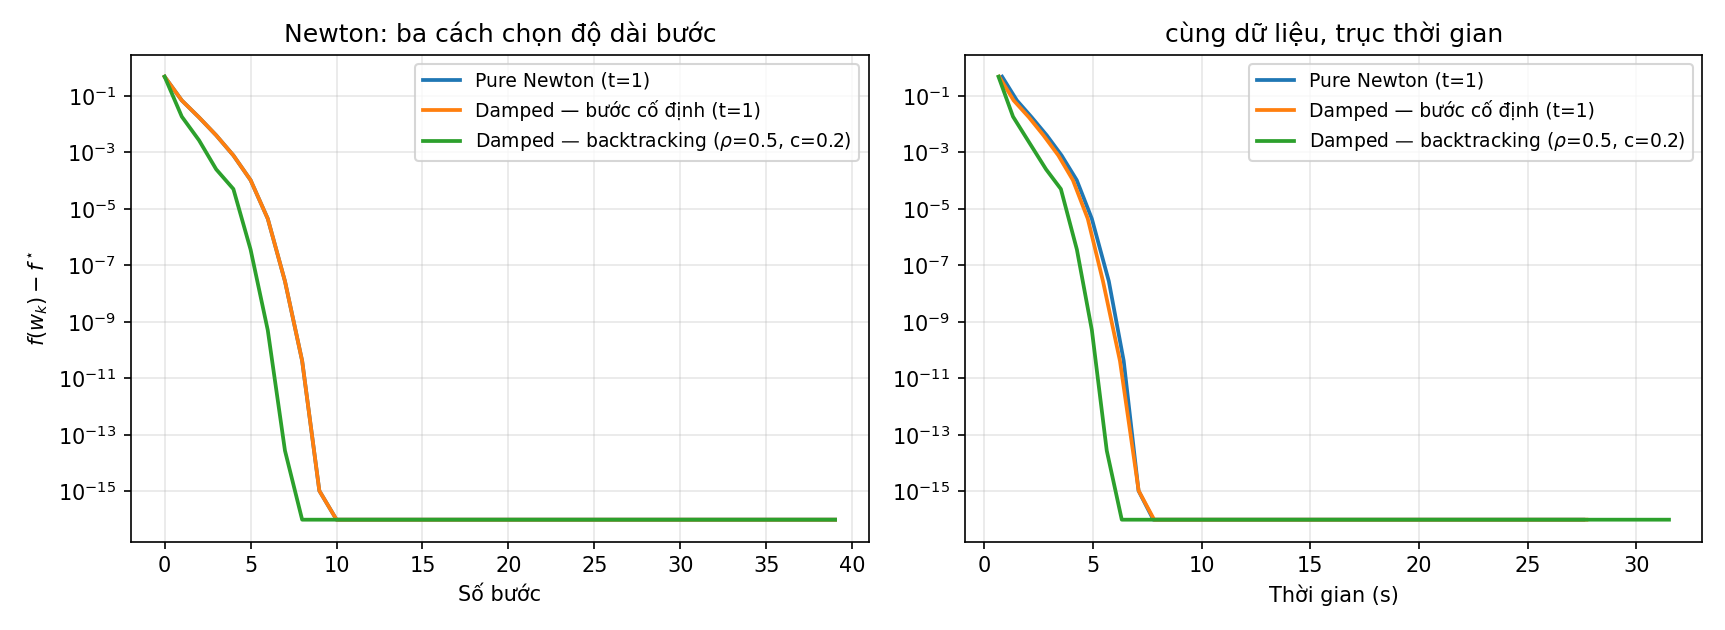
\includegraphics[width=0.94\linewidth]{tune_cmp_newton}}{}
  \end{center}
  \vspace{-2pt}
  {\scriptsize\nx{} (40 vòng, mỗi cách ở tham số đã dò được ở mục 4.3--4.4)}
  \begin{itemize}\scriptsize\itemsep=1pt
    \item Cả ba gần như \textbf{trùng nhau}: pure Newton đã đủ tốt khi khởi tạo gần nghiệm, damping
          không mua thêm được gì đáng kể.
    \item Trái ngược hẳn với GD ở slide trước, nơi ba cách chọn bước cách nhau cả bậc độ lớn. Lý do:
          hướng Newton đã mang sẵn thông tin độ cong, nên độ dài bước không còn là chỗ quyết định.
    \item Damping chỉ thật sự thiết yếu khi khởi tạo \emph{ở xa} --- xem mục 4.6.
  \end{itemize}
\end{frame}

\begin{frame}{4. KẾT QUẢ: DÒ THAM SỐ BẰNG THỬ VÀ SAI}{4.6. Newton — pure và damped khi khởi tạo ở xa nghiệm}
  \begin{center}
    \IfFileExists{../artifacts/figures/newton_init_ridge.png}
      {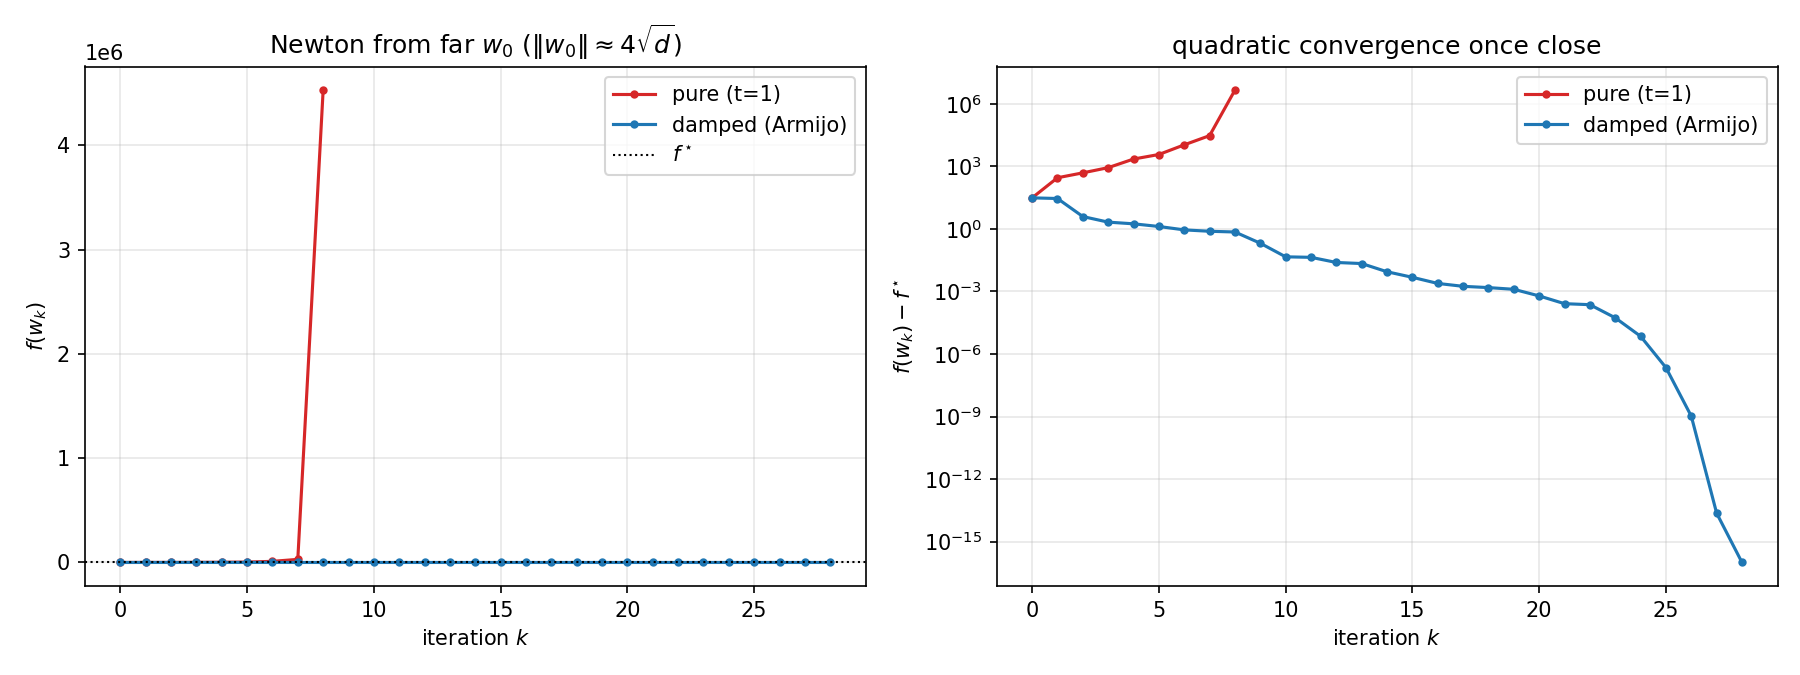
\includegraphics[width=0.80\linewidth]{newton_init_ridge}}{}
  \end{center}
  \vspace{-2pt}
  {\scriptsize\nx{} pure Newton ($t=1$) từ điểm khởi tạo xa bị \textbf{vọt lố} rồi \textbf{chết hẳn},
  không phải chỉ dao động --- đúng điều kiện Kantorovich $h_0\le\frac12$ (mục 2.5). Cơ chế đo được:
  sau 8 bước $\norm{w}$ leo tới $\num{5.1e6}$, mọi sigmoid \textbf{bão hòa} nên
  $S=\mathrm{diag}(p_i(1-p_i))\to0$; hệ số chặn \emph{không} có $\lambda$ đỡ (mục 5.1) nên Hessian
  mất hẳn độ cong và Cholesky \textbf{thất bại thật sự} --- dừng vì \emph{không giải được hệ}, không
  phải vì hết ngân sách. Damped Newton từ \emph{cùng} điểm đó cần \textbf{29 bước}. Damping vì thế
  \textbf{không phải tùy chọn}: khác biệt là chạy được hay không, chứ không phải nhanh hay chậm.}
\end{frame}

\begin{frame}{4. KẾT QUẢ: DÒ THAM SỐ BẰNG THỬ VÀ SAI}{4.7. GD --- dò độ dài bước cố định: thô rồi tinh}
  \begin{center}
    {\large\color{accent}\textbf{$\rightarrow$ Chọn $t = 0{,}4$}}
  \end{center}
  \vspace{-6pt}
  \begin{center}
    \IfFileExists{../artifacts/figures/tune_gd_fixed.png}
      {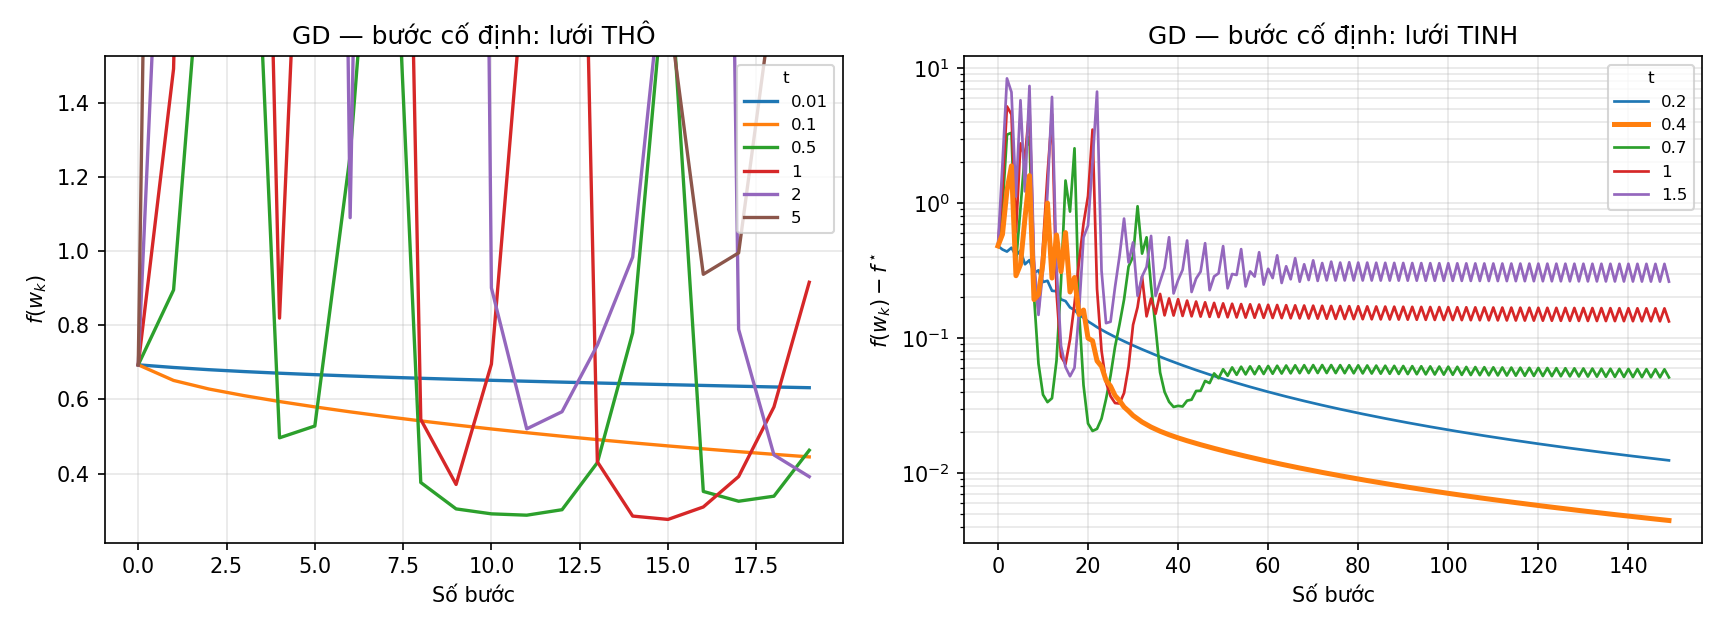
\includegraphics[width=0.76\linewidth]{tune_gd_fixed}}{}
  \end{center}
  \vspace{-2pt}
  {\scriptsize\nx{} \textbf{lưới thô ở đây CHỈ SAI}, và đó là điều đáng nói nhất. Sau 20 vòng nó
  xếp $t=2$ tốt nhất ($0{,}179$), trên cả $0{,}1$ ($0{,}233$) và $0{,}5$ ($0{,}251$). Nhưng lưới
  tinh 150 vòng lật lại: $t=1{,}5$ cho $0{,}262$, $t=1$ cho $0{,}133$, còn
  $t=\mathbf{0{,}4}$ cho $\mathbf{4{,}5\times10^{-3}}$ --- hơn $t=1$ \textbf{30 lần}. $t=2$ gấp 14
  lần ngưỡng $2/L=0{,}142$ nên nó \emph{dao động}; ở đúng vòng thứ 20 nó tình cờ rơi vào pha thấp.
  Bài học: một tầng lưới không đủ, và ngân sách ngắn có thể xếp hạng ngược. Đáng chú ý: $0{,}4$ vẫn
  gấp \textbf{2{,}8 lần} ngưỡng đơn điệu $2/L$ (mục 5.2) --- đơn điệu là \emph{đủ} chứ không
  \emph{cần}.}
\end{frame}

\begin{frame}{4. KẾT QUẢ: DÒ THAM SỐ BẰNG THỬ VÀ SAI}{4.8. GD --- dò $(\rho, c)$ của backtracking: hai trục, hai câu trả lời}
  \begin{center}
    \IfFileExists{../artifacts/figures/tune_gd_bt_grid.png}
      {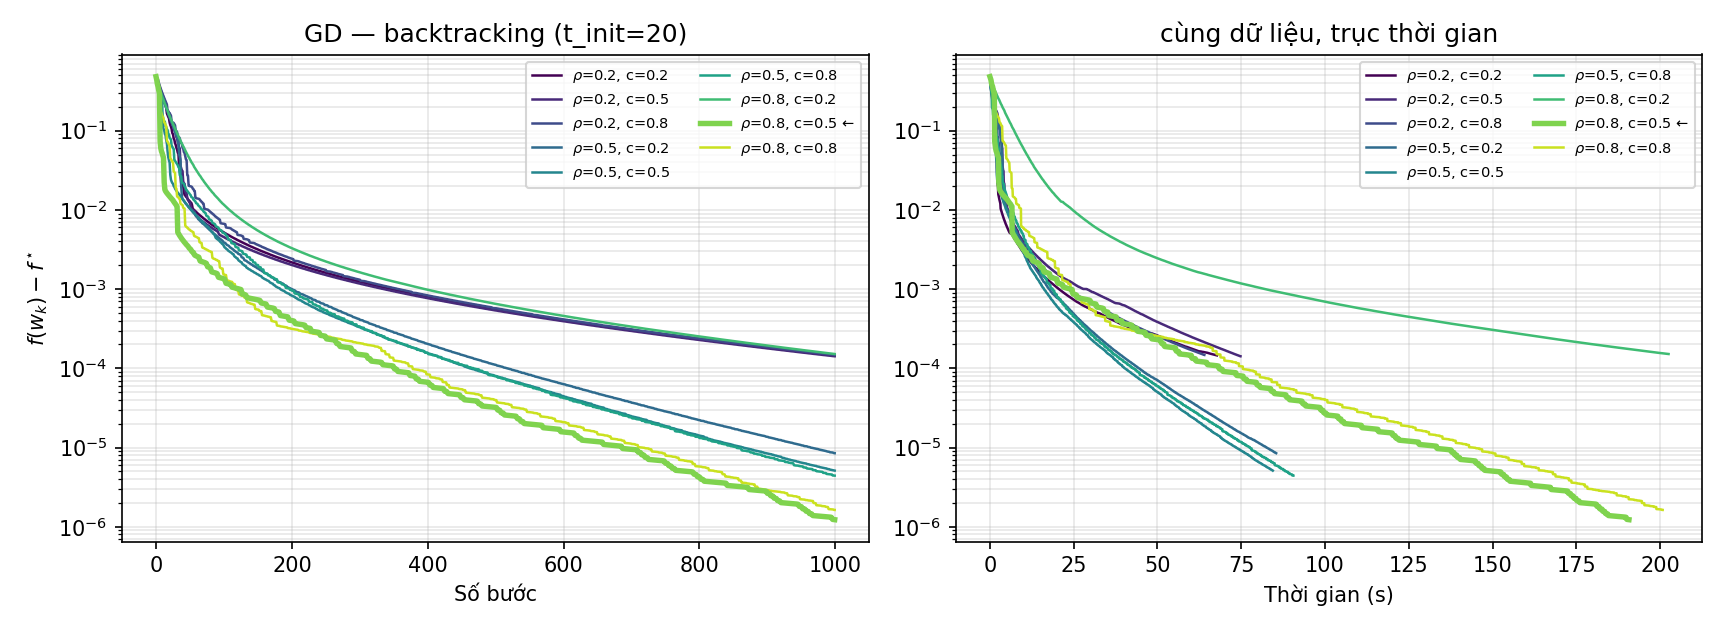
\includegraphics[width=0.64\linewidth]{tune_gd_bt_grid}}{}
  \end{center}
  \vspace{-4pt}
  {\scriptsize\nx{}}
  \begin{itemize}\scriptsize\itemsep=1pt
    \item Chín cấu hình, \num{1000} vòng mỗi cấu hình. Ngân sách dài \emph{không} xóa được mâu
          thuẫn --- nó cho thấy đây là \textbf{biên Pareto thật}: $\rho$ điều khiển cả hai trục
          cùng lúc (co chậm $\Rightarrow$ bước dài hơn $\Rightarrow$ chính xác hơn, nhưng tốn nhiều
          lần tính $f$ hơn), còn $c$ gần như không ảnh hưởng.
    \item \textbf{Chọn $\rho=\mathbf{0{,}8}$, $c=\mathbf{0{,}5}$ theo trục độ chính xác}:
          $\num{1.2e-6}$, tốt nhất lưới --- hơn $(0{,}5;0{,}5)$ \textbf{4,2 lần} và hơn
          $\rho=0{,}2$ tới \textbf{115 lần}. Giá phải trả: \num{190.7}s so với \num{81.7}s.
    \item Vì sao chọn trục này: mục 4.14 so \emph{các thuật toán} ở \textbf{cùng số vòng}, nên mỗi
          thuật toán phải mang tham số cho \emph{nghiệm tốt nhất} của nó, không phải nghiệm rẻ
          nhất. (Góc tệ nhất vẫn là $\rho=0{,}8$, $c=0{,}2$: vừa chậm nhất \num{192.3}s vừa kém
          nhất $\num{1.5e-4}$.)
  \end{itemize}
\end{frame}

\begin{frame}{4. KẾT QUẢ: DÒ THAM SỐ BẰNG THỬ VÀ SAI}{4.9. GD --- backtracking thật sự chọn bước nào?}
  \begin{center}
    \IfFileExists{../artifacts/figures/tune_step_trace_gd.png}
      {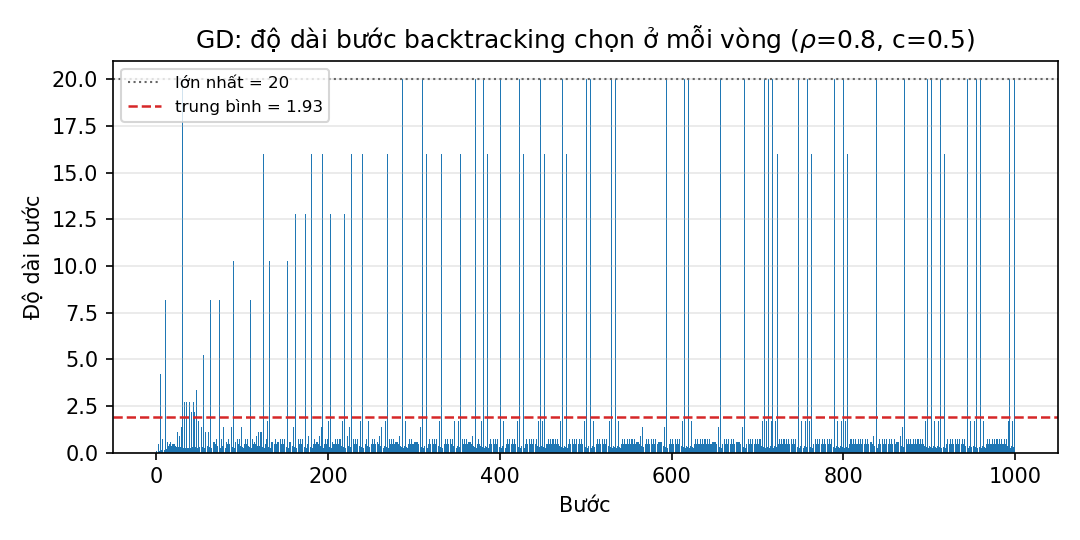
\includegraphics[width=0.62\linewidth]{tune_step_trace_gd}}{}
  \end{center}
  \vspace{-4pt}
  {\scriptsize\nx{}}
  \begin{itemize}\scriptsize\itemsep=1pt
    \item Trung bình $\mathbf{1{,}932}$ --- backtracking \emph{tự tìm ra} một bước gấp
          \textbf{4,8 lần} bước cố định tốt nhất ($0{,}4$), và còn biết lúc nào nên bước dài.
    \item \textbf{$t_{\text{init}}=20$ có lúc được chấp nhận nguyên vẹn} (bước lớn nhất $=20$),
          trong khi $\rho=0{,}5$ không bao giờ vượt quá $10$. Co chậm hơn không chỉ dò \emph{tinh}
          hơn --- nó còn \emph{với tới} được những bước dài mà $\rho$ lớn bỏ lỡ. Đó là nguồn gốc
          của $\num{1.2e-6}$ so với $\num{5.1e-6}$.
    \item Hình này trả lời câu hỏi tự nhiên nhất về backtracking --- nó có thật sự đổi bước không,
          hay chỉ luôn lấy $t_{\text{init}}$ --- mà bảng số không trả lời được.
  \end{itemize}
\end{frame}

\begin{frame}{4. KẾT QUẢ: DÒ THAM SỐ BẰNG THỬ VÀ SAI}{4.10. AGD --- dò độ dài bước cố định}
  \begin{center}
    {\large\color{accent}\textbf{$\rightarrow$ Chọn $t = 0{,}3$}}
  \end{center}
  \vspace{-6pt}
  \begin{center}
    \IfFileExists{../artifacts/figures/tune_gd_accel.png}
      {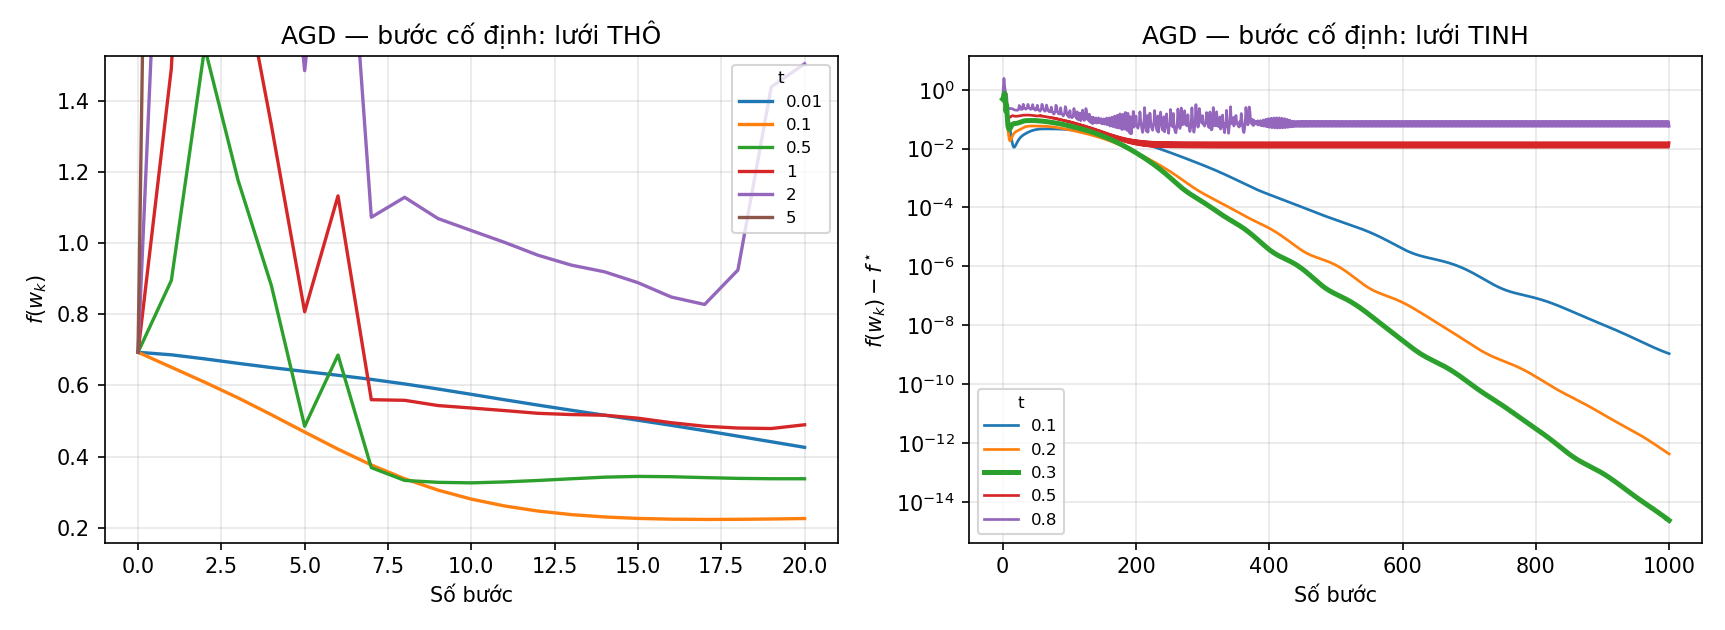
\includegraphics[width=0.70\linewidth]{tune_gd_accel}}{}
  \end{center}
  \vspace{-2pt}
  {\scriptsize\nx{} $\beta=(\sqrt\kappa-1)/(\sqrt\kappa+1)$, lược đồ lồi mạnh
  của~\cite{nesterov2018lectures}. Khác GD ở mục 4.7, lưới thô ở đây \emph{chỉ đúng vùng}
  ($t=0{,}1$ thắng với $1{,}4\times10^{-2}$), và lưới tinh --- chạy \textbf{\num{1000} vòng} ---
  tinh chỉnh lên $t=\mathbf{0{,}3}$: $\num{2.3e-15}$, hơn $t=0{,}2$ ($\num{4.2e-13}$)
  \textbf{180 lần}, còn $t=0{,}5$ sập xuống $\num{1.6e-2}$.
  \textbf{Bước tốt nhất phụ thuộc ngân sách}: ở 150 vòng thì $0{,}2$ mới thắng. Ta chọn theo
  \num{1000} vòng vì money plot và mục 4.12--4.13 đều chạy ở đó. Lưu ý $0{,}3$ là giá trị lớn nhất
  \emph{trước vách sập} --- tối ưu thật nằm trong $(0{,}3;\,0{,}5)$, lưới này không tách được.}
\end{frame}

\begin{frame}{4. KẾT QUẢ: DÒ THAM SỐ BẰNG THỬ VÀ SAI}{4.11. AGD --- lược đồ momentum $(k-2)/(k+1)$: dò bước}
  \begin{center}
    {\large\color{accent}\textbf{$\rightarrow$ Chọn $t = 0{,}3$}}
  \end{center}
  \vspace{-6pt}
  \begin{center}
    \IfFileExists{../artifacts/figures/tune_agd_k.png}
      {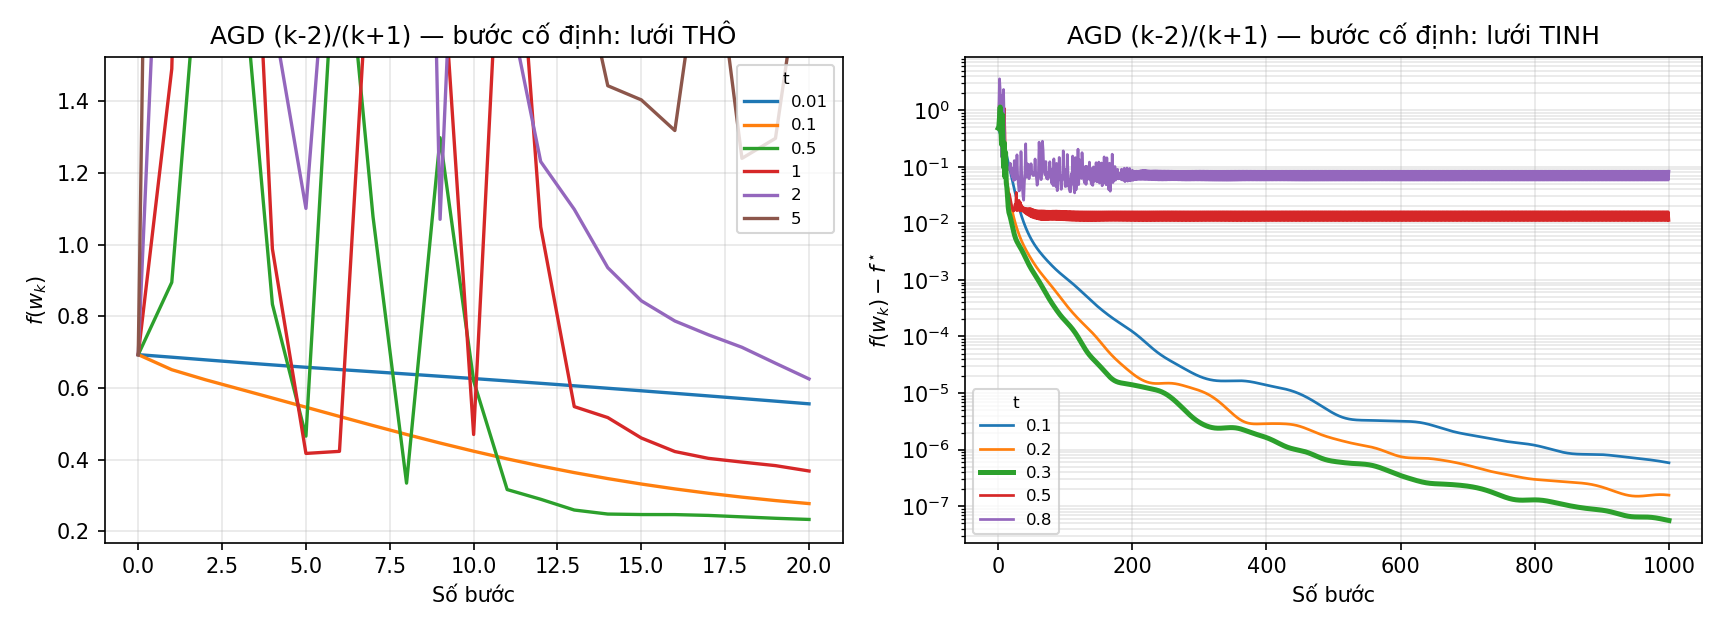
\includegraphics[width=0.68\linewidth]{tune_agd_k}}{}
  \end{center}
  \vspace{-2pt}
  {\scriptsize\nx{} lược đồ Nesterov cho hàm lồi \emph{thường}~\cite{beck2009fista}:
  $v=w_{k-1}+\frac{k-2}{k+1}(w_{k-1}-w_{k-2})$, $w_k=v-t\nabla f(v)$, tốc độ $O(1/k^2)$.
  Hệ số momentum ở đây \textbf{không chứa hằng số nào của bài toán} --- không $L$, không $\mu$ ---
  nên $t$ là tham số tự do thật sự, dò tay được. Lưới tinh đặt \emph{đúng bằng} lưới của mục 4.10 để
  hai bảng so trực tiếp, và cùng chạy \textbf{\num{1000} vòng}. Các giá trị tách nhau rõ:
  $0{,}1\to\num{5.8e-7}$, $0{,}2\to\num{1.6e-7}$, $t=\mathbf{0{,}3}\to\mathbf{\num{5.6e-8}}$, rồi
  $0{,}5$ \emph{sập} xuống $\num{1.1e-2}$. Lưới thô lại chỉ sai một lần nữa --- sau 20 vòng nó xếp
  $t=0{,}5$ đầu bảng, đúng giá trị mà lưới tinh loại 5 bậc.
  \textbf{Trùng đúng $t=0{,}3$ của mục 4.10}, nên mục 4.12 so hai lược đồ ở \emph{cùng một bước}.}
\end{frame}

\begin{frame}{4. KẾT QUẢ: DÒ THAM SỐ BẰNG THỬ VÀ SAI}{4.12. AGD --- hai lược đồ momentum: ai thắng tùy ngân sách}
  \begin{center}
    \IfFileExists{../artifacts/figures/agd_schemes.png}
      {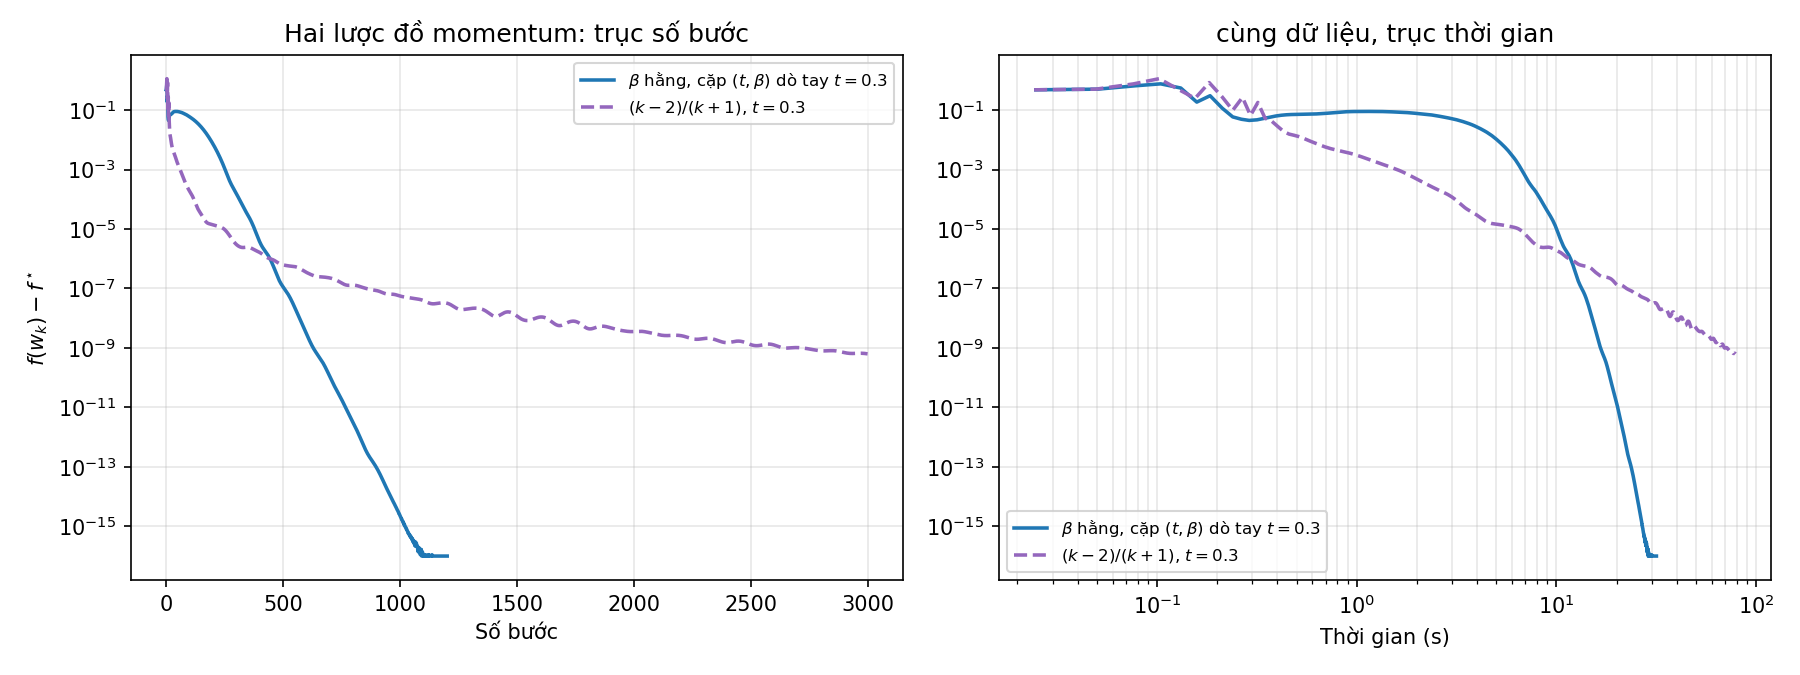
\includegraphics[width=0.50\linewidth]{agd_schemes}}{}
  \end{center}
  \vspace{-2pt}
  {\scriptsize\nx{} hai lược đồ, mỗi cái ở bước \textbf{dò tay} tốt nhất của chính nó
(cả hai đều $t=0{,}3$ --- mục 4.10 và 4.11 dò ra
  cùng một bước, nên chênh lệch dưới đây là do \textbf{momentum thuần túy}), trần \num{3000} vòng.
  Chưa dùng $1/L$ ở đây --- bước theo lý thuyết là chuyện của mục 5.}
  \begin{itemize}\scriptsize\itemsep=1pt
    \item \textbf{$(k-2)/(k+1)$ thắng ở giai đoạn đầu}: momentum khởi động từ $0$ rồi tăng dần
          nên không vọt lố, trong khi $\beta$ hằng đặt $0{,}966$ ngay từ vòng 1 và có một
          \emph{bướu} rõ trong $\sim$100 vòng đầu.
    \item \textbf{Nhưng nó không hội tụ}: \num{3000} vòng vẫn còn $6{,}3\times10^{-10}$, vì
          $O(1/k^2)$ là \emph{dưới tuyến tính} --- nó không dùng tới tính lồi mạnh. $\beta$ hằng
          vượt hẳn lên từ \textbf{vòng \num{445}} (đo, không ước lượng bằng mắt --- và từ đó không
          bị cắt lại) rồi rơi thẳng đứng, hội tụ sau \textbf{\num{1202} vòng / \num{31.7}s}.
    \item Rút ra: $(k-2)/(k+1)$ dùng được khi \textbf{không ước lượng nổi $\mu$}; hàm thật sự lồi
          mạnh thì $\beta$ hằng thắng đường dài. \emph{Adaptive restart}~\cite{odonoghue2015restart}
          --- đặt lại $k$ mỗi khi $f$ tăng --- gỡ được đánh đổi này: nó đạt tốc độ tuyến tính mà
          \textbf{không cần biết $\mu$}. Ta \textbf{chưa} cài, đây là hướng mở rộng tự nhiên.
  \end{itemize}
\end{frame}

\begin{frame}{4. KẾT QUẢ: DÒ THAM SỐ BẰNG THỬ VÀ SAI}{4.13. GD và AGD --- so sánh bốn cách chọn bước}
  \begin{center}
    \IfFileExists{../artifacts/figures/tune_cmp_gd.png}
      {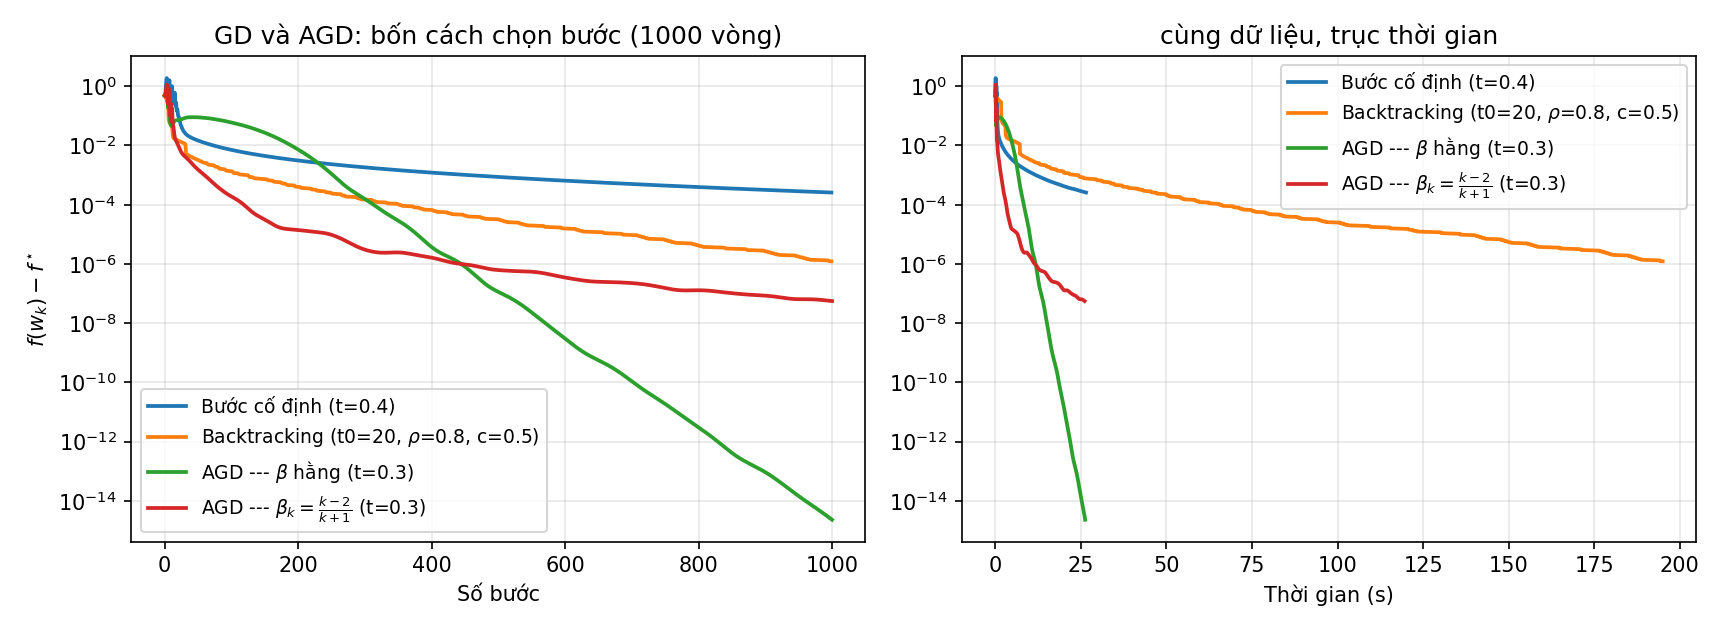
\includegraphics[width=0.54\linewidth]{tune_cmp_gd}}{}
  \end{center}
  \vspace{-2pt}
  {\scriptsize\nx{} (\num{1000} vòng, mỗi cấu hình ở tham số đã dò ở mục 4.7--4.11)}
  \begin{itemize}\scriptsize\itemsep=1pt
    \item \textbf{AGD $\beta$ hằng thắng tuyệt đối}: $\num{2.3e-15}$, hơn GD bước cố định
          ($\num{2.6e-4}$) \textbf{11 bậc} --- mà \emph{cùng thời gian} (\num{26.3}s so với
          \num{26.1}s). Momentum không tốn thêm gì: cả hai đúng một gradient mỗi vòng.
    \item \textbf{Đảo chiều so với ngân sách ngắn.} Ở 150 vòng AGD còn \emph{thua} GD
          ($\num{2.2e-2}$ so với $\num{4.5e-3}$). Lợi thế $\sqrt\kappa$ là phát biểu
          \emph{tiệm cận}, và \num{1000} vòng là chỗ nó hiện ra --- cùng một cặp thuật toán, đổi
          ngân sách là đổi kết luận.
    \item \textbf{Backtracking} ($\rho=0{,}8$, mục 4.8): tốt hơn bước cố định \textbf{210 lần}
          ($\num{2.6e-4}\to\num{1.2e-6}$) nhưng tốn \textbf{7,4 lần thời gian} (\num{195.0}s so với
          \num{26.5}s). Theo trục thời gian nó thua \emph{cả hai} AGD rất xa --- và vẫn thua AGD
          $\beta$ hằng \textbf{9 bậc} về độ chính xác, dù đã đắt gấp 7 lần.
    \item \textbf{Hai lược đồ momentum} chạy ở \emph{cùng} $t=0{,}3$: $\beta$ hằng hơn
          $(k-2)/(k+1)$ ($\num{5.6e-8}$) \textbf{7 bậc}. Cùng bước, cùng thời gian --- khác biệt
          hoàn toàn do momentum, khớp mục 4.12: qua vòng 445 thì lồi mạnh thắng.
  \end{itemize}
\end{frame}

\begin{frame}{4. KẾT QUẢ: DÒ THAM SỐ BẰNG THỬ VÀ SAI}{4.14. SGD --- dò lịch bước cho từng cỡ mini-batch}
  \begin{center}
    \IfFileExists{../artifacts/figures/tune_sgd_schedules.png}
      {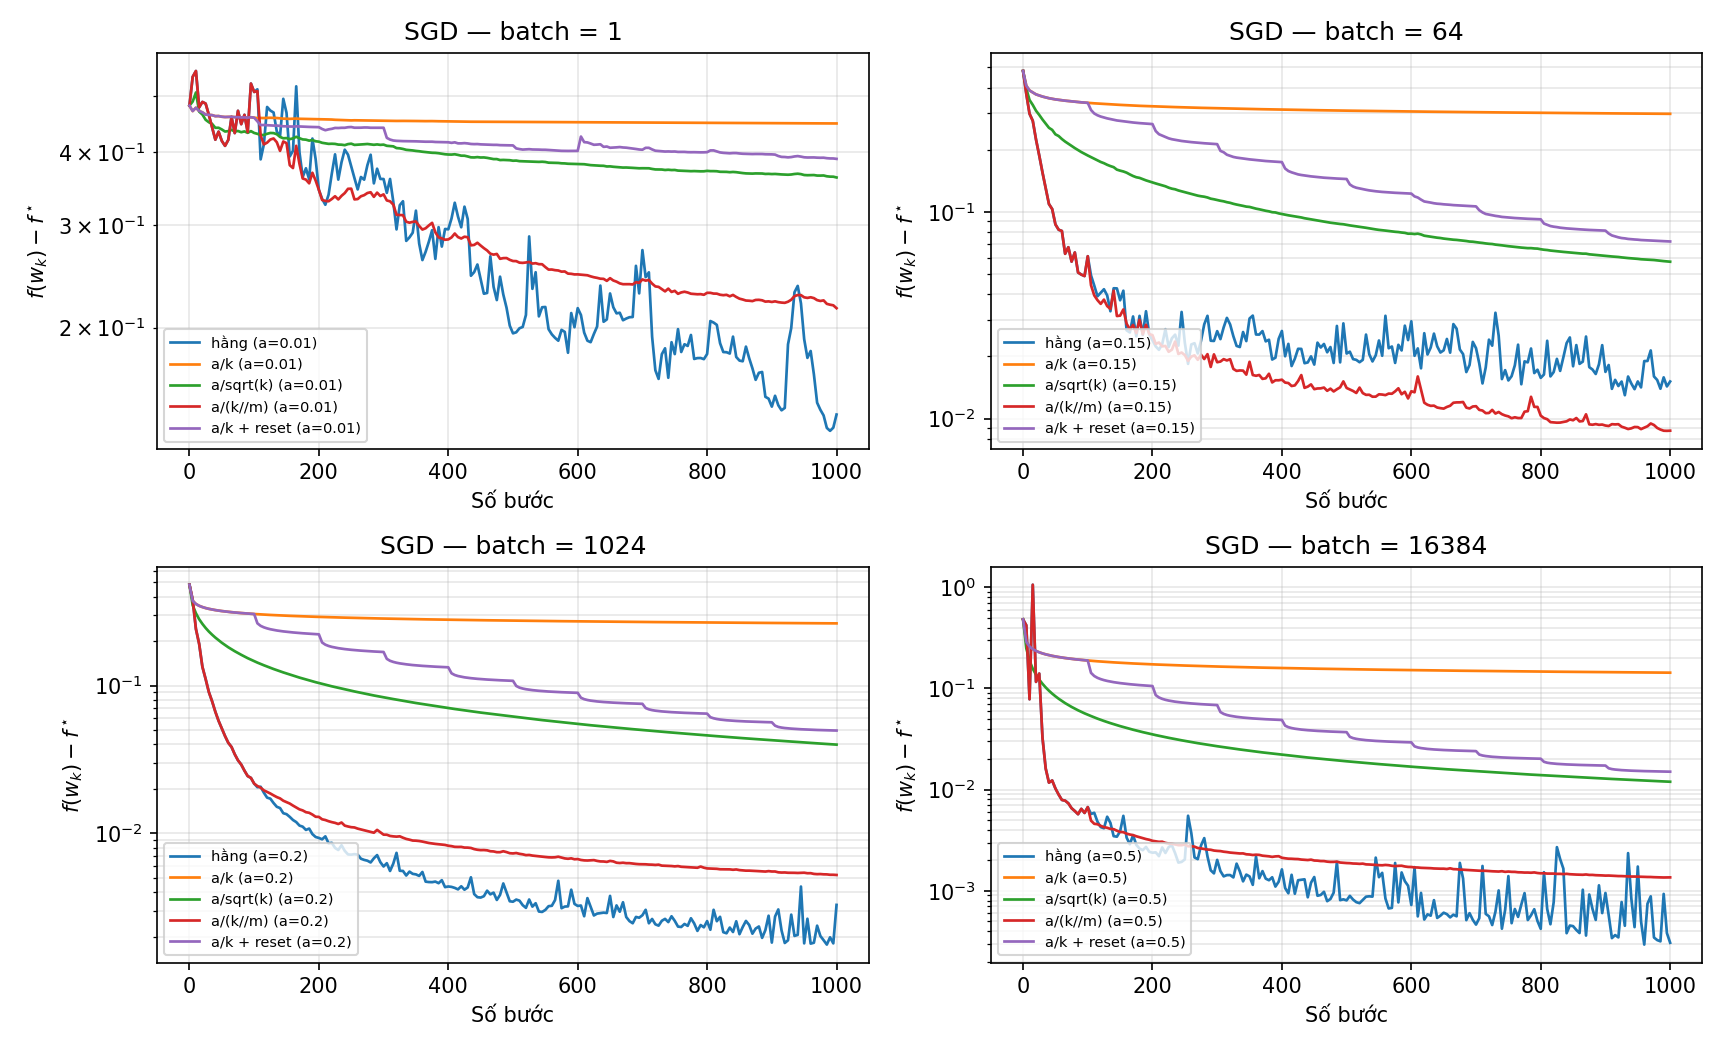
\includegraphics[width=0.62\linewidth]{tune_sgd_schedules}}{}
  \end{center}
  \vspace{-4pt}
  {\scriptsize\nx{} (1000 bước mini-batch) $\alpha$ tốt nhất \textbf{tăng theo batch}:
  $0{,}01\to0{,}15\to0{,}2\to0{,}5$ khi $b:1\to\num{64}\to\num{1024}\to\num{16384}$.
  \textbf{$\alpha/k$ luôn tệ nhất} (thua 1--2 bậc ở mọi cỡ batch) dù nó \emph{thỏa}
  Robbins--Monro --- thỏa điều kiện là chuyện tiệm cận, còn trong ngân sách hữu hạn thì bước đã tắt
  trước khi kịp đi tới đâu. Với batch lớn, \textbf{bước hằng tốt nhất}.}
\end{frame}

\begin{frame}{4. KẾT QUẢ: DÒ THAM SỐ BẰNG THỬ VÀ SAI}{4.15. SGD --- batch càng lớn càng tốt?}
  \begin{center}
    \IfFileExists{../artifacts/figures/tune_sgd_batches.png}
      {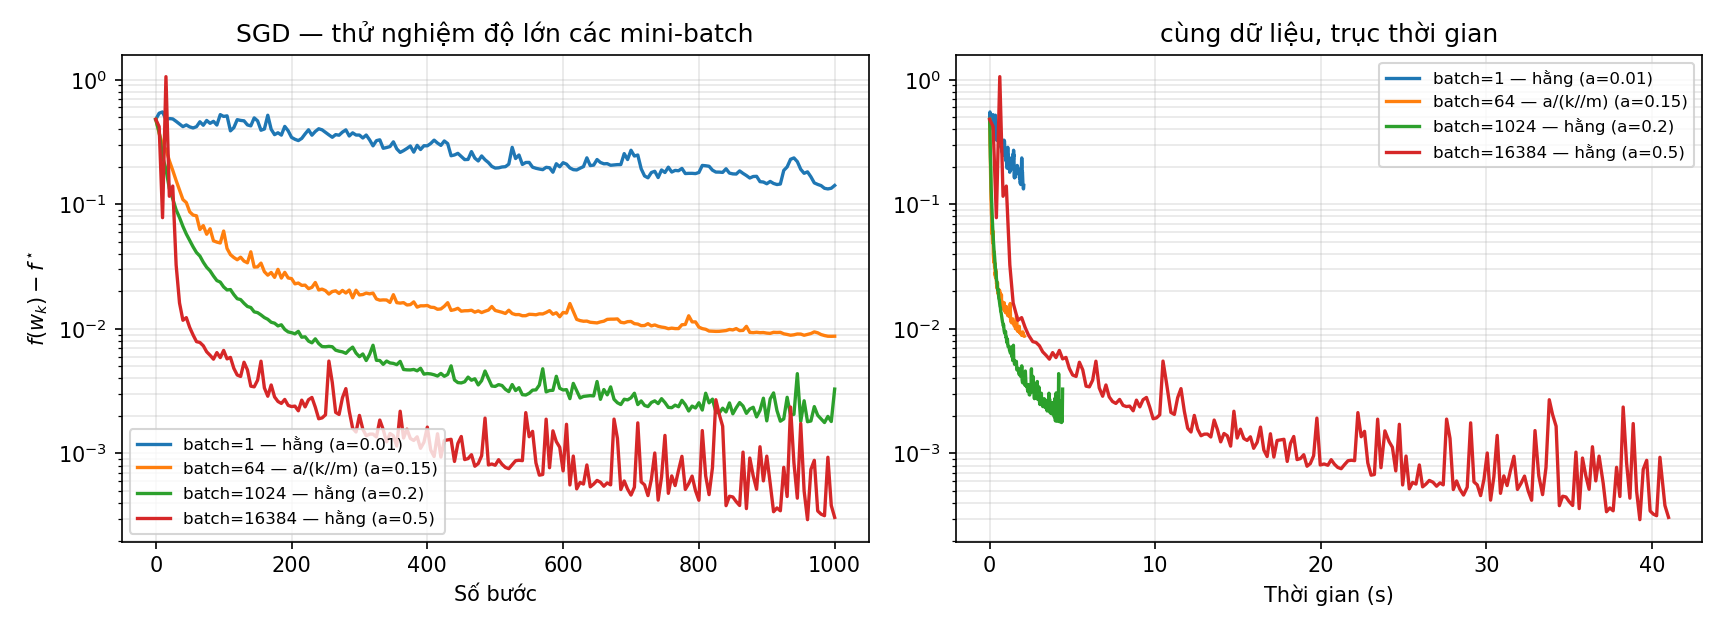
\includegraphics[width=0.86\linewidth]{tune_sgd_batches}}{}
  \end{center}
  \vspace{-4pt}
  {\scriptsize\nx{}}
  \begin{itemize}\scriptsize\itemsep=1pt
    \item Theo \textbf{số bước}: đúng là càng lớn càng tốt, đơn điệu --- $b=1$ dừng ở
          $1{,}4\times10^{-1}$, $b=\num{16384}$ xuống $3{,}1\times10^{-4}$, cách nhau \textbf{3 bậc}.
    \item Theo \textbf{thời gian} thì \emph{không}: $b=\num{1024}$ đạt $\sim\!2\times10^{-3}$ sau
          $4{,}5$s, còn $b=\num{16384}$ cần \num{20}s mới tới cùng mức. Trong 5 giây đầu, batch vừa
          phải \textbf{dẫn trước} batch lớn.
    \item Lý do: so ở cùng \emph{số bước} là không công bằng --- một bước của $b=\num{16384}$ đọc
          nhiều gấp 16 lần. Trục thời gian mới quy về cùng đơn vị công việc.
  \end{itemize}
\end{frame}

\begin{frame}{4. KẾT QUẢ: DÒ THAM SỐ BẰNG THỬ VÀ SAI}{4.16. Tổng hợp: tham số đã dò được của từng thuật toán}
  \vspace{-2pt}
  \begin{center}\tiny
  \begin{tabular}{lllcc}
    \toprule
    Thuật toán & Tham số chọn & Dò ở & So \emph{trong} họ & \textbf{Vào 4.16--4.18}\\
    \midrule
    Newton --- bước cố định   & $t=1$ (pure)               & 4.2  & 4.4 & \\
    Newton --- backtracking   & $t_{init}=2$, $\rho=0{,}5$, $c=0{,}2$ & 4.3 & 4.4 & \\
    \midrule
    GD --- bước cố định       & $t=0{,}4$                  & 4.6  & 4.13 & \textbf{\checkmark}\\
    GD --- backtracking       & $t_{init}=20$, $\rho=0{,}8$, $c=0{,}5$ & 4.7 & 4.13 & \\
    \midrule
    AGD --- $\beta$ hằng      & $t=0{,}3\Rightarrow\beta=0{,}966$ & 4.9 & 4.11, 4.13 & \textbf{\checkmark}\\
    AGD --- $\beta_k=\frac{k-2}{k+1}$ & $t=0{,}3$          & 4.10 & 4.11, 4.13 & \\
    \midrule
    SGD                       & $\eta_0=0{,}2$, $b=\num{1024}$, hằng & 4.13--4.14 & --- & \textbf{\checkmark}\\
    \bottomrule
  \end{tabular}
  \end{center}
  \vspace{1pt}
  {\scriptsize\nx{}}
  \begin{itemize}\scriptsize\itemsep=1pt
    \item \textbf{Mục 4.16--4.18 chỉ mang MỘT cấu hình cho mỗi họ} --- bảy dòng ở đây là bảy
          \emph{biến thể chọn bước}, còn phần so sánh sau đó trả lời câu hỏi khác: họ thuật toán
          nào thắng. Ba dòng không đánh dấu đã được so \emph{trong họ} ở mục 4.5, 4.12 và 4.14.
    \item \textbf{Newton ở mục 4.17--4.19 là damped Newton + backtracking với $\rho=0{,}5$,
          $c=10^{-4}$}, \emph{không} phải cặp $c=0{,}2$ ở dòng 2: $c=0{,}2$ là điều kiện Armijo
          chặt, gần nghiệm thì nhiễu số học làm nó luôn trượt nên bước co về $0$ --- chạm trần 100
          vòng / \num{95}s mà không đạt $\norm{\nabla f}<10^{-14}$, so với 15 vòng / \num{10.4}s
          của mặc định. Cùng lần chạy đó sinh ra $f^\star$ nên nó phải \emph{chứng nhận được}.
    \item \textbf{Ba lần trục đo quyết định câu trả lời}: Newton so bằng \emph{số vòng};
          GD-backtracking chọn giữa \emph{độ chính xác} và \emph{thời gian} (biên Pareto); SGD đọc
          theo \emph{thời gian}. Và không tham số nào trùng cận lý thuyết ($0{,}4$ so với
          $2/L=0{,}142$; $0{,}3$ so với $1/L=0{,}071$) --- mục 5 chứng minh vì sao.
  \end{itemize}
\end{frame}

\begin{frame}{4. KẾT QUẢ: DÒ THAM SỐ BẰNG THỬ VÀ SAI}{4.17. So sánh cả bảy cấu hình --- theo số bước}
  \begin{center}
    \IfFileExists{../artifacts/figures/money7_iter.png}
      {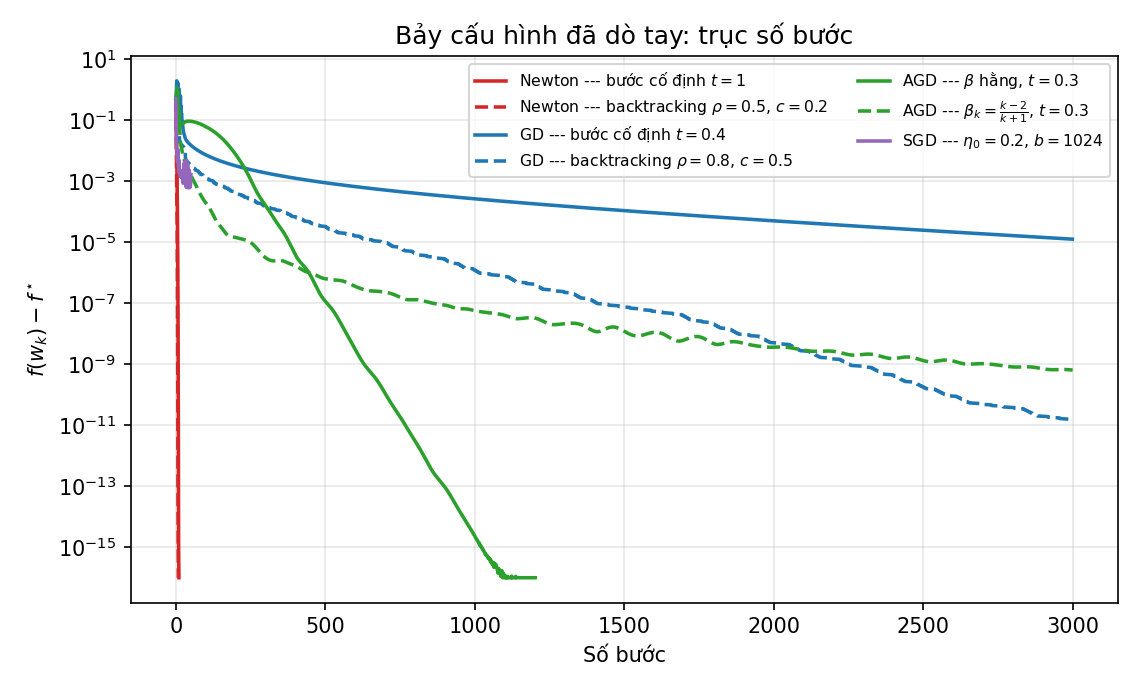
\includegraphics[width=0.50\linewidth]{money7_iter}}{}
  \end{center}
  \vspace{-2pt}
  {\scriptsize\nx{} bảy cấu hình của bảng 4.16, \emph{không} cấu hình nào lấy từ nơi khác. Cùng
  tiêu chí dừng $\norm{\nabla f}<10^{-10}$, cùng trần \num{3000} vòng, cùng $f^\star$ của mục 4.2.
  Màu = họ thuật toán, nét = cách chọn bước.}
  \begin{itemize}\scriptsize\itemsep=1pt
    \item \textbf{Hai đường Newton dựng đứng ở mép trái}: 10 và \textbf{8} vòng. Backtracking dò
          tay \emph{nhanh hơn} pure Newton --- $c=0{,}2$ cho phép nhận bước dài hơn $1$ ở pha đầu.
    \item \textbf{Chỉ 3/7 đạt tiêu chí dừng}: hai Newton và AGD $\beta$ hằng (\num{1202} vòng).
          Bốn cấu hình còn lại chạm trần.
    \item \textbf{Trong cùng một họ, cách chọn bước đổi kết quả tới 6 bậc}: GD $\num{1.2e-5}$ so
          với $\num{1.5e-11}$; AGD $0$ so với $\num{6.3e-10}$. Chênh lệch \emph{trong} họ lớn hơn
          chênh lệch \emph{giữa} vài họ.
  \end{itemize}
\end{frame}

\begin{frame}{4. KẾT QUẢ: DÒ THAM SỐ BẰNG THỬ VÀ SAI}{4.18. So sánh cả bảy cấu hình --- theo thời gian}
  \begin{columns}[T]
    \begin{column}{0.56\textwidth}
      \IfFileExists{../artifacts/figures/money7_time.png}
        {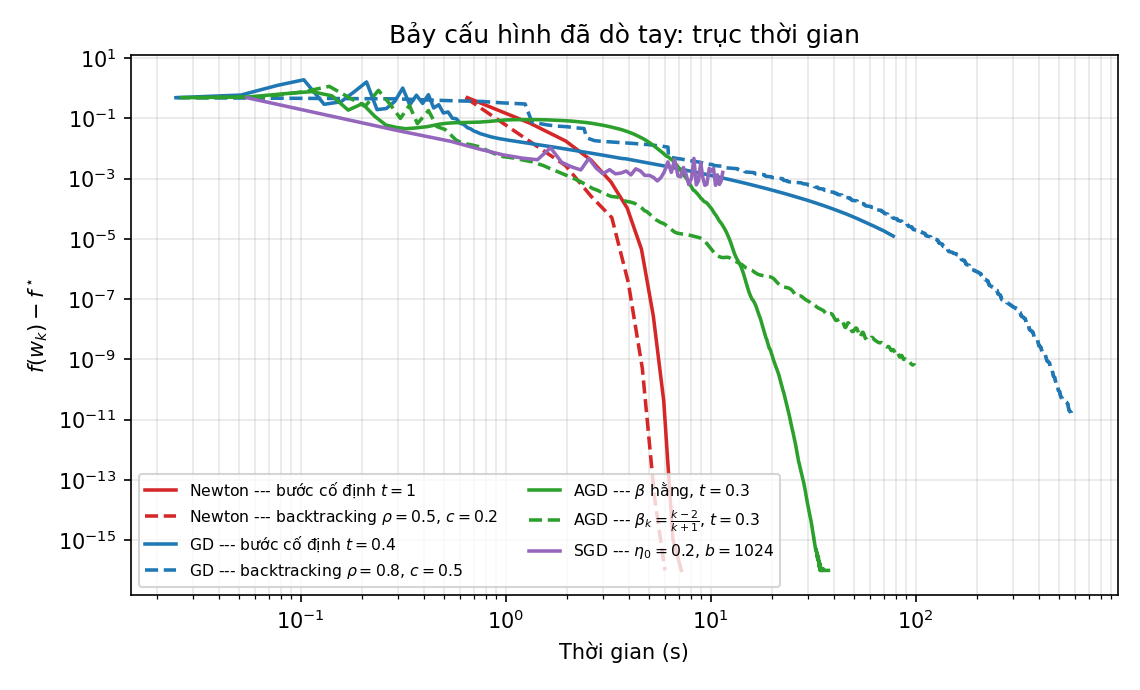
\includegraphics[width=\linewidth]{money7_time}}{}
    \end{column}
    \begin{column}{0.44\textwidth}
      \begin{center}\tiny
      \begin{tabular}{lrrr}
        \toprule
        Cấu hình & Bước & $f-f^\star$ & Giây\\
        \midrule
        Newton bt $(0{,}5;0{,}2)$ & \textbf{8}    & $0$           & \textbf{6{,}0}\\
        Newton $t=1$              & 10            & $0$           & 7{,}2\\
        SGD                       & 50 ep         & $\num{1.6e-3}$& 11{,}4\\
        AGD $\beta$ hằng          & \num{1202}    & $0$           & 37{,}5\\
        GD $t=0{,}4$              & $>$\num{3000} & $\num{1.2e-5}$& 77{,}7\\
        AGD $(k{-}2)/(k{+}1)$     & $>$\num{3000} & $\num{6.3e-10}$& 99{,}1\\
        GD backtracking           & $>$\num{3000} & $\num{1.5e-11}$& 583{,}2\\
        \bottomrule
      \end{tabular}
      \end{center}
    \end{column}
  \end{columns}
  \vspace{-2pt}
  {\scriptsize\nx{}}
  \begin{itemize}\scriptsize\itemsep=1pt
    \item \textbf{Newton thắng cả hai trục} dù mỗi bước của nó đắt nhất: $0{,}75$s một bước, gấp
          \textbf{24 lần} một bước AGD --- nhưng cần ít hơn \textbf{150 lần} số bước.
    \item \textbf{Đổi trục là đổi hạng.} GD-backtracking chính xác thứ ba ($\num{1.5e-11}$) nhưng
          \emph{chậm nhất bảng} (\num{583.2}s, gấp 7,5 lần GD bước cố định); ngược lại SGD thứ ba
          về thời gian nhưng bét về độ chính xác.
    \item Toàn bộ luận điểm của bài trong một hình: \textbf{chi phí mỗi vòng} nhân \textbf{số
          vòng} mới ra thời gian, và hai thừa số đó đi ngược chiều nhau.
  \end{itemize}
\end{frame}

\begin{frame}{4. KẾT QUẢ: DÒ THAM SỐ BẰNG THỬ VÀ SAI}{4.19. Đối chiếu với thư viện \texttt{scikit-learn}}
  \scriptsize
  Khớp đúng dạng hàm mục tiêu: \texttt{scikit-learn} tối thiểu $\tfrac12\norm{w}^2+C\sum_i\ell_i$,
  hàm của nhóm lấy \emph{trung bình} $\Rightarrow C=1/(n\lambda)$; hệ số chặn không bị phạt ở cả
  hai phía.
  \begin{center}\scriptsize
  \begin{tabular}{lccc}
    \toprule
    Solver & $f-f^\star$ & Số bước & Thời gian (s)\\
    \midrule
    \texttt{sklearn lbfgs}           & $2{,}2\times10^{-13}$ & \num{225}   & \textbf{\num{3.31}}\\
    \texttt{sklearn newton-cholesky} & $2{,}8\times10^{-17}$ & \num{10}    & \num{6.84}\\
    Newton (nhóm tự cài)             & $0$                   & \num{11}    & \num{10.21}\\
    SGD (nhóm tự cài)$^\dagger$      & $1{,}6\times10^{-3}$  & 51 epoch    & \num{10.60}\\
    Accelerated GD (nhóm tự cài)     & $5{,}6\times10^{-17}$ & \num{1335}  & \num{39.7}\\
    GD (nhóm tự cài)$^\dagger$       & $2{,}1\times10^{-13}$ & \num{20000} & \num{540.9}\\
    \texttt{sklearn saga}            & $1{,}2\times10^{-11}$ & \num{5000}  & \num{852}\\
    \bottomrule
  \end{tabular}
  \end{center}
  {\scriptsize $^\dagger$ chạm trần ngân sách, chưa đạt $\norm{\nabla f}<10^{-11}$. Mọi dòng
  "nhóm tự cài" chạy ở tham số đã dò ở mục 4.16.}
  {\scriptsize\nx{}}
  \begin{itemize}\scriptsize\itemsep=1pt
    \item Newton của nhóm (11 bước) khớp \texttt{newton-cholesky} (10 bước) tới độ chính xác máy:
          chênh lệch \num{10.21}s so với \num{6.84}s chỉ đến từ cài đặt (BLAS/Cython),
          \emph{không} từ thuật toán~\cite{sklearn}.
    \item \textbf{Đảo chiều so với bài toán nhỏ:} ở $d=39$ Newton nhanh nhất, ở $d=415$
          \textbf{\texttt{lbfgs} thắng} (\num{3.31}s) --- quasi-Newton tốn $O(nd)$ mỗi vòng và
          không bao giờ dựng Hessian, nên 225 vòng rẻ hơn 10 vòng đắt.
    \item \textbf{GD tới được cùng độ chính xác --- nhưng mất \num{541}s}, gấp \textbf{163 lần}
          \texttt{lbfgs} cho cùng $\sim$$10^{-13}$: cái giá của tốc độ tuyến tính khi
          $\kappa=\num{14069}$. Còn \textbf{SGD dừng ở $1{,}6\times10^{-3}$}, kém 10 bậc, ở đúng mốc thời
          gian của Newton --- rẻ để tới \emph{gần}, không phải tới nghiệm.
  \end{itemize}
\end{frame}

% =====================================================================
\section{Hằng số Lipschitz và chọn bước theo lý thuyết}
% =====================================================================

\begin{frame}[plain]
  \label{sec:5}%
  \begin{center}{\Large\color{accent}\textbf{5. HẰNG SỐ LIPSCHITZ VÀ CHỌN BƯỚC}}\\[4pt]
  {\small Mục 4 chọn bước bằng cách \emph{dò tay}. Mục này hỏi: lý thuyết nói gì,
  và nó cách thực nghiệm bao xa?}\end{center}
\end{frame}

\begin{frame}{5. HẰNG SỐ LIPSCHITZ VÀ CHỌN BƯỚC THEO LÝ THUYẾT}{5.1. Hàm phạt Ridge và ba hằng số $L,\ \mu,\ \kappa$}
  \small
  Với hàm phạt Ridge, $\nabla^2 f(w)=\dfrac1n X^\top S X+\lambda I$. Do $0<p(1-p)\le\frac14$:
  \[
    \lambda\,I\ \preceq\ \nabla^2 f(w)\ \preceq\ \Big(\underbrace{\tfrac{1}{4n}\lambda_{\max}(X^\top X)+\lambda}_{L}\Big) I
  \]
  \begin{itemize}
    \item $\mu\ge\lambda>0$: hàm \textbf{lồi mạnh} $\Rightarrow$ nghiệm $\wstar$ \textbf{tồn tại và duy nhất}.
    \item $L$: hằng số \textbf{trơn} (Lipschitz của gradient) $\Rightarrow$ quyết định độ dài bước tối đa.
    \item $\kappa=L/\mu$: \textbf{số điều kiện} — xuất hiện trong tốc độ hội tụ của mọi thuật toán bậc nhất.
  \end{itemize}
  \vspace{2pt}
  {\footnotesize\textit{Chính xác hơn:} hệ số chặn \textbf{không bị phạt}, nên số hạng Ridge thực ra là
  $\lambda\,\mathrm{diag}(r)$ với một số $0$ ở vị trí hệ số chặn. Bất đẳng thức bên trái chỉ đúng trên các
  tọa độ bị phạt; theo hướng hệ số chặn, độ cong là $\frac1n\sum_i p_i(1-p_i)\to0$ khi $\norm{w}\to\infty$.
  Vậy $f$ lồi mạnh trên mọi \textbf{tập mức bị chặn}, không phải toàn cục --- tại nghiệm đo được
  $\mu_\star=\num{1.00e-3}$, tức gần \emph{đúng bằng} $\lambda$: ở $d=415$ số hạng Ridge là thứ duy
  nhất chống đỡ hướng cong yếu nhất. Điều này \emph{không} vô hại: xem mục 4.6; chứng minh cận $L$ ở mục 5.2.}
\end{frame}

\begin{frame}{5. HẰNG SỐ LIPSCHITZ VÀ CHỌN BƯỚC THEO LÝ THUYẾT}{5.2. Chứng minh cận $L$, và vì sao ngưỡng lại là $2/L$}
  \footnotesize
  \textbf{Bước 1 --- chặn độ cong theo từng mẫu.} Với $p=\sigma(z)$ thì $p(1-p)$ đạt cực đại tại
  $p=\frac12$, nên $0<p_i(1-p_i)\le\frac14$ với mọi $i$ và mọi $w$.

  \textbf{Bước 2 --- từ đó chặn dạng toàn phương.} Với mọi $v\ne0$:
  \[
    v^\top\!\Big(\tfrac1n X^\top S X\Big)v=\frac1n\sum_i p_i(1-p_i)\,(x_i^\top v)^2
    \ \le\ \frac{1}{4n}\sum_i (x_i^\top v)^2=\frac14\,v^\top\!\Big(\tfrac1n X^\top X\Big)v
    \ \le\ \frac{\lambda_{\max}\!\big(\tfrac1n X^\top X\big)}{4}\,\norm{v}^2 .
  \]
  Cộng số hạng Ridge $\lambda\,\mathrm{diag}(r)\preceq\lambda I$ được
  $\ \nabla^2f(w)\preceq L\,I\ $ với $\ L=\frac14\lambda_{\max}(\frac1nX^\top X)+\lambda$,
  \textbf{đúng với mọi $w$}.

  \textbf{Bước 3 --- $\nabla^2f\preceq LI$ chính là tính $L$-trơn.} Khai triển Taylor bậc hai với phần
  dư Lagrange cho \emph{bổ đề giảm}: $f(y)\le f(x)+\nabla f(x)^\top(y-x)+\frac{L}{2}\norm{y-x}^2$.

  \textbf{Bước 4 --- thay $y=x-t\nabla f(x)$} vào bổ đề giảm:
  \[
    f\big(x-t\nabla f(x)\big)\ \le\ f(x)-t\Big(1-\frac{tL}{2}\Big)\norm{\nabla f(x)}^2 .
  \]
  Hệ số $t(1-tL/2)$ dương $\iff t<2/L$. \textbf{Đó là toàn bộ nguồn gốc của ngưỡng $2/L$}: nó bảo
  đảm $f$ \emph{giảm} ở mỗi bước, chứ không nói gì về việc bước nào \emph{tốt nhất}.
  \vspace{2pt}

  {\scriptsize\nx{} cả bốn bước đều lấy bất đẳng thức theo hướng \emph{an toàn} (bước 1 lấy
  $\frac14$ cho mọi mẫu dù $p_i(1-p_i)$ nhỏ hơn nhiều khi rời $w_0$; bước 2 lấy $\lambda_{\max}$
  cho mọi hướng), nên $2/L$ là điều kiện \textbf{đủ}, không \textbf{cần}. Đo được: GD dò tay ra
  $0{,}4$, gấp $\mathbf{2{,}8}$ lần $2/L$ (mục 4.7); AGD ở cặp dò tay $t=0{,}3$ cần
  \textbf{\num{1202} vòng / \num{31.7}s} so với \num{2400} vòng / \num{63.1}s ở bước $1/L$ ---
  nhanh hơn \textbf{2,0 lần} trên cả hai trục. Cái \emph{phá} AGD là đổi $t$ mà \textbf{giữ nguyên} $\beta$, không
  phải rời khỏi $1/L$.}
\end{frame}

\begin{frame}{5. HẰNG SỐ LIPSCHITZ VÀ CHỌN BƯỚC THEO LÝ THUYẾT}{5.3. Xác định hằng số trơn $L$ --- bốn đường, một con số}
  \begin{center}
    \IfFileExists{../artifacts/figures/tune_L.png}
      {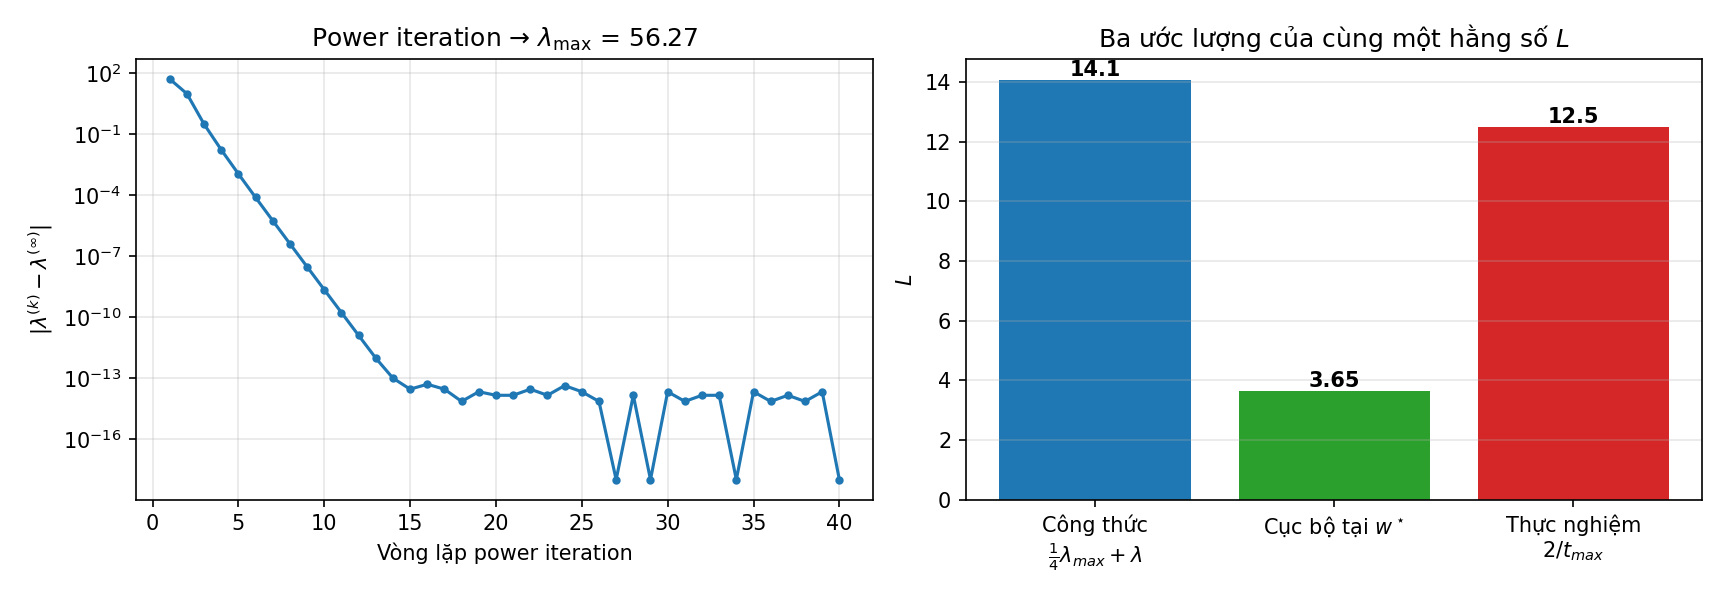
\includegraphics[width=0.86\linewidth]{tune_L}}{}
  \end{center}
  \vspace{-4pt}
  {\scriptsize\nx{}}
  \begin{itemize}\scriptsize\itemsep=1pt
    \item \textbf{Công thức} (dùng $0<p(1-p)\le\frac14$): $L=\frac14\lambda_{\max}(\frac1nX^\top X)+\lambda
          =\num{14.07}$. Đúng với \emph{mọi} $w$ --- an toàn nhưng bi quan.
    \item \textbf{Power iteration} cho cùng $\lambda_{\max}=\num{56.27}$ nhưng chỉ tốn $O(nd)$ mỗi vòng
          thay vì $O(nd^2{+}d^3)$ của \texttt{eigvalsh}, và hội tụ tới độ chính xác máy sau
          \textbf{15 vòng}. Đây là cách duy nhất còn rẻ khi $d$ lớn hơn nữa.
    \item \textbf{Độ cong cục bộ} tại $\wstar$: $L_\star=\num{3.65}$ --- nhỏ hơn \textbf{3{,}9 lần},
          vì tại nghiệm thì $p(1-p)$ đã rời xa $\frac14$.
    \item \textbf{Thực nghiệm}: bước cố định lớn nhất mà GD còn \emph{giảm đơn điệu} nằm trong
          khoảng $(0{,}16;\,0{,}20)$, trong khi lý thuyết nói ngưỡng là $2/L=\num{0.142}$.
          Cận lý thuyết chỉ bi quan $1{,}1$--$1{,}4$ lần --- \textbf{khá chặt}.
  \end{itemize}
\end{frame}

\begin{frame}{5. HẰNG SỐ LIPSCHITZ VÀ CHỌN BƯỚC THEO LÝ THUYẾT}{5.4. Ba vùng độ dài bước quanh $2/L$ và $2/\lambda$}
  \begin{center}
    \IfFileExists{../artifacts/figures/three_regimes_ridge.png}
      {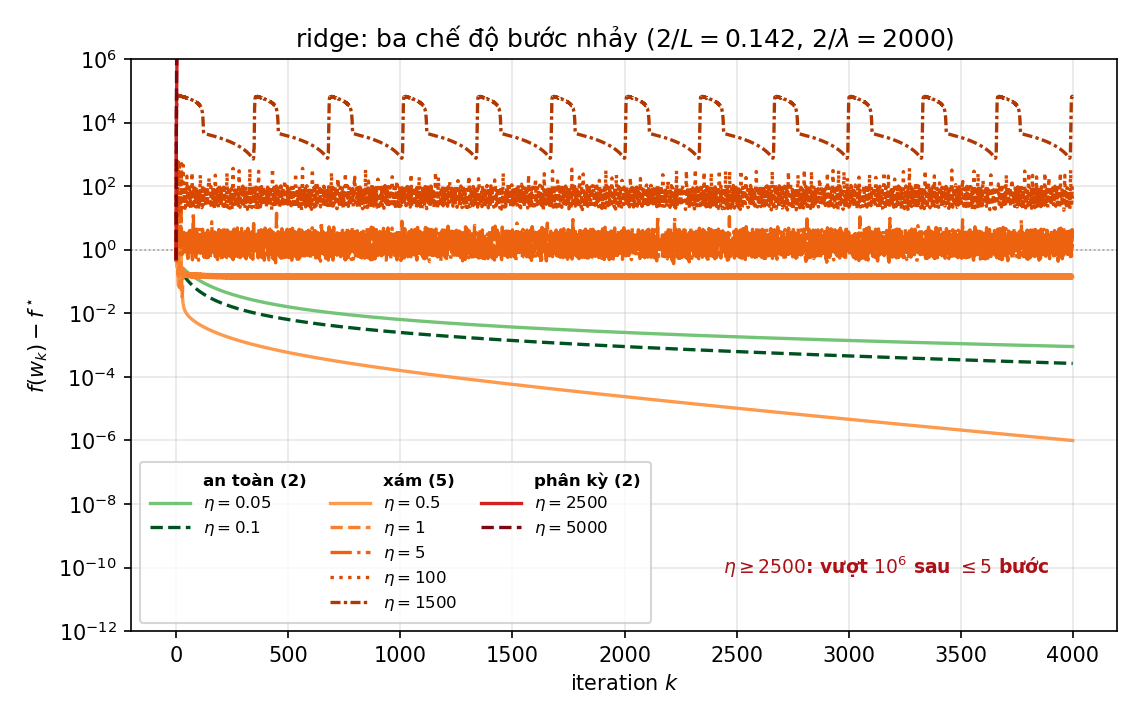
\includegraphics[width=0.58\linewidth]{three_regimes_ridge}}{}
  \end{center}
  \vspace{-4pt}
  {\scriptsize\nx{} ba vùng, mỗi vùng một cột chú giải.
  \textcolor{regimeSafe}{$t<2/L=\num{0.142}$} (xanh): giảm \textbf{đơn điệu} đúng lý thuyết ---
  nhưng \emph{chậm nhất} hình.
  \textcolor{regimeGray}{$2/L<t<2/\lambda$} (cam, 5 đường): \textbf{dao động} nhưng hữu hạn, và
  $\eta=0{,}5$ về tới $10^{-6}$ --- nhanh hơn cả hai đường "an toàn"; bước dò tay $t=0{,}4$ của
  mục 4.7 nằm ở đây.
  \textcolor{regimeDiv}{$t>2/\lambda=\num{2000}$} (đỏ): \textbf{phân kỳ} thật sự, vượt $10^{6}$
  sau $\le5$ bước nên chạy khỏi khung ngay ở mép trái.}
\end{frame}

\begin{frame}{5. HẰNG SỐ LIPSCHITZ VÀ CHỌN BƯỚC THEO LÝ THUYẾT}{5.5. Kiểm chứng tốc độ lý thuyết: GD tỉ lệ $\kappa$, AGD tỉ lệ $\sqrt\kappa$}
  \begin{columns}[T]
    \begin{column}{0.52\textwidth}
      \IfFileExists{../artifacts/figures/kappa_sweep_ridge.png}
        {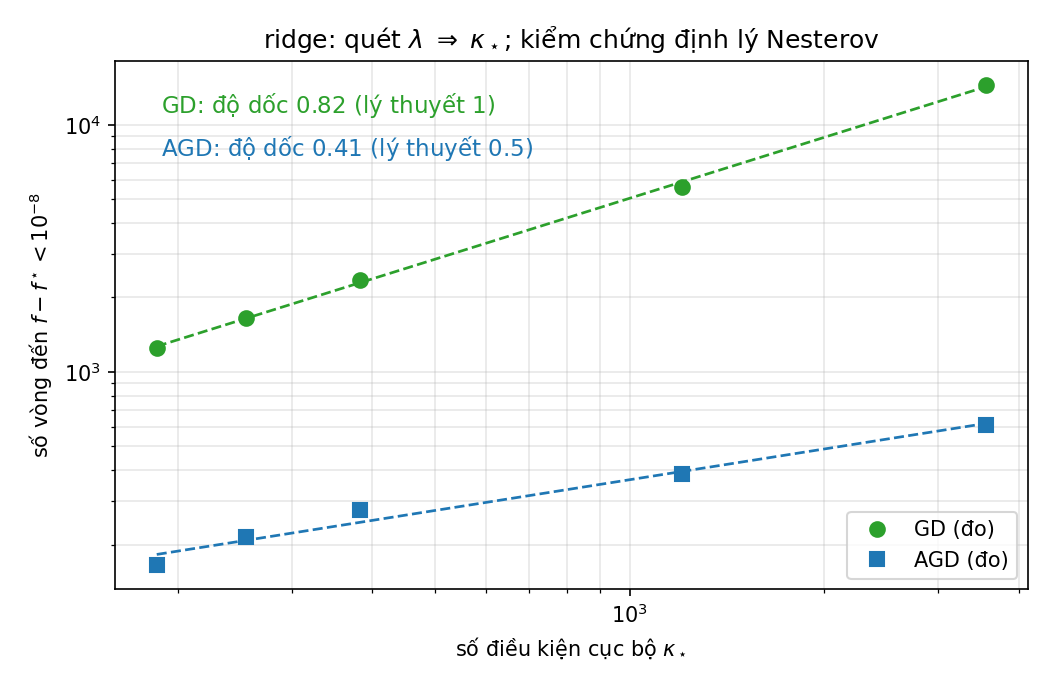
\includegraphics[width=\linewidth]{kappa_sweep_ridge}}{}
    \end{column}
    \begin{column}{0.48\textwidth}\scriptsize
      Thay đổi $\lambda$ để $\kappa_\star$ trải $\sim$1{,}3 bậc, đếm số bước tới $f-f^\star<10^{-8}$:
      \begin{center}\tiny
      \begin{tabular}{crr}
        \toprule
        $\kappa_\star$ & GD & AGD\\
        \midrule
        \num{185.5}  & \num{1252}  & \num{165}\\
        \num{255.0}  & \num{1658}  & \num{214}\\
        \num{382.6}  & \num{2362}  & \num{275}\\
        \num{1204.5} & \num{5613}  & \num{386}\\
        \num{3559.9} & \num{14541} & \num{609}\\
        \bottomrule
      \end{tabular}
      \end{center}
      \nx{}
      \begin{itemize}\scriptsize\itemsep=0pt
        \item Độ dốc log--log: GD \textbf{\num{0.819}}, AGD \textbf{\num{0.413}} --- cả hai thấp hơn
              lý thuyết ($1$ và $\tfrac12$) vì đó là \textbf{cận trên}.
        \item Nhưng \textbf{tỉ số} là $0{,}819/0{,}413=\mathbf{1{,}98}$, gần đúng bằng $2$ --- đây
              mới là điều $\kappa$ vs $\sqrt\kappa$ tiên đoán.
        \item $\kappa_\star$ tăng 19 lần: GD tốn thêm \textbf{11{,}6} lần bước, AGD \textbf{3{,}7}.
      \end{itemize}
    \end{column}
  \end{columns}
  {\scriptsize Đo trên mẫu \num{15000}/\num{75026} dòng --- $\kappa$ là tính chất của hình học đặc
  trưng, không phải của cỡ mẫu (lệch $2{,}4\%$), mà GD cần $O(\kappa\log\frac1\epsilon)$ vòng.}
\end{frame}

% =====================================================================
\section{Mở rộng: họ Ada và họ Adam}
% =====================================================================

\begin{frame}{6. MỘT SỐ THUẬT TOÁN TỐI ƯU KHÁC}{6.1. Họ các thuật toán Ada}
  \label{sec:6}%
  \footnotesize
  \begin{columns}[T]
    \begin{column}{0.5\textwidth}
      \textbf{AdaGrad} \textit{(Adaptive Gradient)}~\cite{duchi2011adagrad}:
      \[
        G_k=G_{k-1}+g_k^2,\qquad
        w_{k+1}=w_k-\frac{\eta}{\sqrt{G_k}+\epsilon}\,g_k
      \]
      Trong đó $g_k$ là gradient tại bước $k$, $G_k$ lưu tổng bình phương các gradient trước đó,
      $\epsilon$ là hằng số nhỏ tránh chia cho 0. Mọi phép toán thực hiện \emph{theo từng tọa độ}.
      \vspace{6pt}

      \textbf{AdaDelta:} tương tự RMSprop nhưng bổ sung $\Delta w_k$ nên \textbf{không cần} tham số
      độ dài bước:
      \[
        \Delta w_k=-\frac{\sqrt{E[\Delta w^2]_{k-1}+\epsilon}}{\sqrt{E[g^2]_k+\epsilon}}\;g_k
      \]
    \end{column}
    \begin{column}{0.5\textwidth}
      \textbf{RMSprop:} hạn chế của AdaGrad là $G_k$ chỉ tăng, làm độ dài bước tắt dần.
      RMSprop thay $G_k$ bằng trung bình trọng số của bình phương gradient:
      \[
        E[g^2]_k=\gamma\,E[g^2]_{k-1}+(1-\gamma)\,g_k^2
      \]
      \vspace{6pt}

      \nx{}
      \begin{itemize}\scriptsize
        \item Bản chất là \textbf{đổi thang đo theo từng tọa độ} — họ hàng rẻ tiền của Newton:
              $O(d)$ mỗi bước thay vì $O(nd^2{+}d^3)$.
        \item Chuẩn hóa $z$-score (mục 3.2) đã cân bằng \emph{thang đo} các cột, nhưng
              \emph{không} cân bằng độ cong cục bộ $p_i(1-p_i)$ — phần việc còn lại này
              chính là chỗ bước thích nghi vẫn giúp được (mục 6.6).
        \item Cận lý thuyết của AdaGrad là $O(1/k)$, yếu hơn tốc độ tuyến tính của GD —
              nhưng đó là \emph{cận trên} cho trường hợp xấu nhất.
      \end{itemize}
    \end{column}
  \end{columns}
\end{frame}

\begin{frame}{6. MỘT SỐ THUẬT TOÁN TỐI ƯU KHÁC}{6.2. Họ các thuật toán Adam}
  \footnotesize
  \begin{columns}[T]
    \begin{column}{0.48\textwidth}
      \textbf{Adam} \textit{(Adaptive Moment Estimation)}~\cite{kingma2015adam} $=$ RMSprop $+$ Momentum:
      \begin{align*}
        m_k&=\beta_1 m_{k-1}+(1-\beta_1)g_k\\
        v_k&=\beta_2 v_{k-1}+(1-\beta_2)g_k^2\\
        \hat m_k&=\frac{m_k}{1-\beta_1^k},\qquad \hat v_k=\frac{v_k}{1-\beta_2^k}\\
        w_{k+1}&=w_k-\frac{\eta}{\sqrt{\hat v_k}+\epsilon}\,\hat m_k
      \end{align*}
      $\beta_1,\beta_2$ là tỷ lệ trọng số của các ước lượng moment (thường là $0{,}9$ và $0{,}999$).
    \end{column}
    \begin{column}{0.52\textwidth}
      \textbf{AdamW} \textit{(Adam with Weight Decay)}~\cite{loshchilov2019adamw}: tách hàm phạt ra khỏi gradient
      \[
        w_{k+1}=w_k-\eta\Big(\tfrac{\hat m_k}{\sqrt{\hat v_k}+\epsilon}+\lambda w_k\Big)
      \]
      \textbf{Nadam:} thay động lượng thường bằng động lượng Nesterov
      \[
        w_{k+1}=w_k-\eta\,\frac{\beta_1\hat m_k+(1-\beta_1)g_k}{\sqrt{\hat v_k}+\epsilon}
      \]
      \textbf{AMSGrad}~\cite{reddi2018amsgrad}: dùng $\hat v_k=\max(\hat v_{k-1},v_k)$ để mẫu số không giảm —
      vá lại chứng minh hội tụ của Adam gốc.
    \end{column}
  \end{columns}
\end{frame}

\begin{frame}{6. MỘT SỐ THUẬT TOÁN TỐI ƯU KHÁC}{6.3. Hai biến thể của Adam --- cơ chế}
  \small
  \textbf{AMSGrad --- kẹp $\hat v_k=\max(\hat v_{k-1},v_k)$.}
  \begin{itemize}\footnotesize
    \item Adam lấy $\hat v_k$ là trung bình trượt, nên mẫu số $\sqrt{\hat v_k}$ \emph{có thể giảm}
          $\Rightarrow$ bước hiệu dụng $\eta/\sqrt{\hat v_k}$ có thể \emph{tăng} trở lại giữa chừng.
          Đó chính là chỗ chứng minh hội tụ của Adam bị thủng.
    \item Phép kẹp lấy max làm $\sqrt{\hat v_k}$ \textbf{không giảm}, nên bước hiệu dụng đơn điệu
          không tăng --- điều kiện kiểu Robbins--Monro được khôi phục. RMSprop \emph{không} có
          tính chất này.
  \end{itemize}
  \vspace{2pt}
  \textbf{AdamW --- weight decay tách rời, và hệ quả không hiển nhiên của nó.}
  \begin{itemize}\footnotesize
    \item Thay vì cộng $\lambda w$ vào gradient, AdamW trừ thẳng $\eta\lambda w$ khỏi $w$. Điểm
          dừng vì thế thỏa $\nabla g(w)+\lambda(\sqrt{\hat v}+\epsilon)\,w=0$, trong khi
          $\arg\min f$ thỏa $\nabla g(w)+\lambda w=0$.
    \item Hai phương trình này chỉ trùng nhau khi $\sqrt{\hat v}+\epsilon=1$. Nói cách khác AdamW
          \textbf{không tối thiểu hóa cùng một hàm mục tiêu} với các thuật toán còn lại --- nó
          không thuộc cùng một cuộc đua.
  \end{itemize}
  \vspace{2pt}
  {\footnotesize\nx{} số đo kiểm chứng cả hai điều trên ở mục 6.8.}
\end{frame}

\begin{frame}{6. MỘT SỐ THUẬT TOÁN TỐI ƯU KHÁC}{6.4. Dò $\eta$ cho cả họ --- cùng một quy trình thô rồi tinh}
  \small
  Cả năm thuật toán dò theo đúng quy trình của mục 4.3: lưới thô cách nhau một bậc 10, rồi lưới
  tinh bao quanh giá trị thắng, rồi nhìn hình mà chọn.
  \begin{center}\small
  \begin{tabular}{lccl}
    \toprule
    & $\eta$ chọn & $f-f^\star$ (150 vòng) & Ghi chú\\
    \midrule
    \textbf{AMSGrad} & \textbf{0{,}2}  & $\mathbf{1{,}2\!\cdot\!10^{-3}}$ & cực tiểu nội\\
    Adam    & \num{0.12} & $4{,}5\!\cdot\!10^{-4}$ & phải nới lưới lên mới ra\\
    AdaGrad & \num{0.3}  & $7{,}0\!\cdot\!10^{-3}$ & cực tiểu nội ngay vòng đầu\\
    AdamW   & \num{0.08} & $5{,}6\!\cdot\!10^{-3}$ & phải nới lưới lên mới ra\\
    RMSprop & \num{0.02} & $5{,}1\!\cdot\!10^{-2}$ & phải nới lưới lên; vẫn tệ nhất họ\\
    \bottomrule
  \end{tabular}
  \end{center}
  \vspace{4pt}
  {\footnotesize\nx{}}
  \begin{itemize}\footnotesize
    \item Vòng dò đầu đặt lưới tinh theo kết quả cũ ở \num{3000} vòng, và \textbf{ba trong năm thuật
          toán chạm mép trên}: ở ngân sách 150 vòng thì bước tối ưu \emph{lớn hơn hẳn}
          (Adam $0{,}01\to0{,}12$, gấp 12 lần).
    \item Nên không thể chép tham số từ một lần chạy khác --- $\eta$ tốt nhất phụ thuộc \textbf{cả
          ngân sách}, không riêng hàm mục tiêu. Cả năm giá trị cuối đều là cực tiểu \emph{nội}.
  \end{itemize}
\end{frame}

\begin{frame}{6. MỘT SỐ THUẬT TOÁN TỐI ƯU KHÁC}{6.5. Dò $\eta$ --- minh họa với AMSGrad}
  \begin{center}
    {\large\color{accent}\textbf{$\rightarrow$ Chọn $\eta = 0{,}2$}}
  \end{center}
  \vspace{-6pt}
  \begin{center}
    \IfFileExists{../artifacts/figures/tune_ada_amsgrad.png}
      {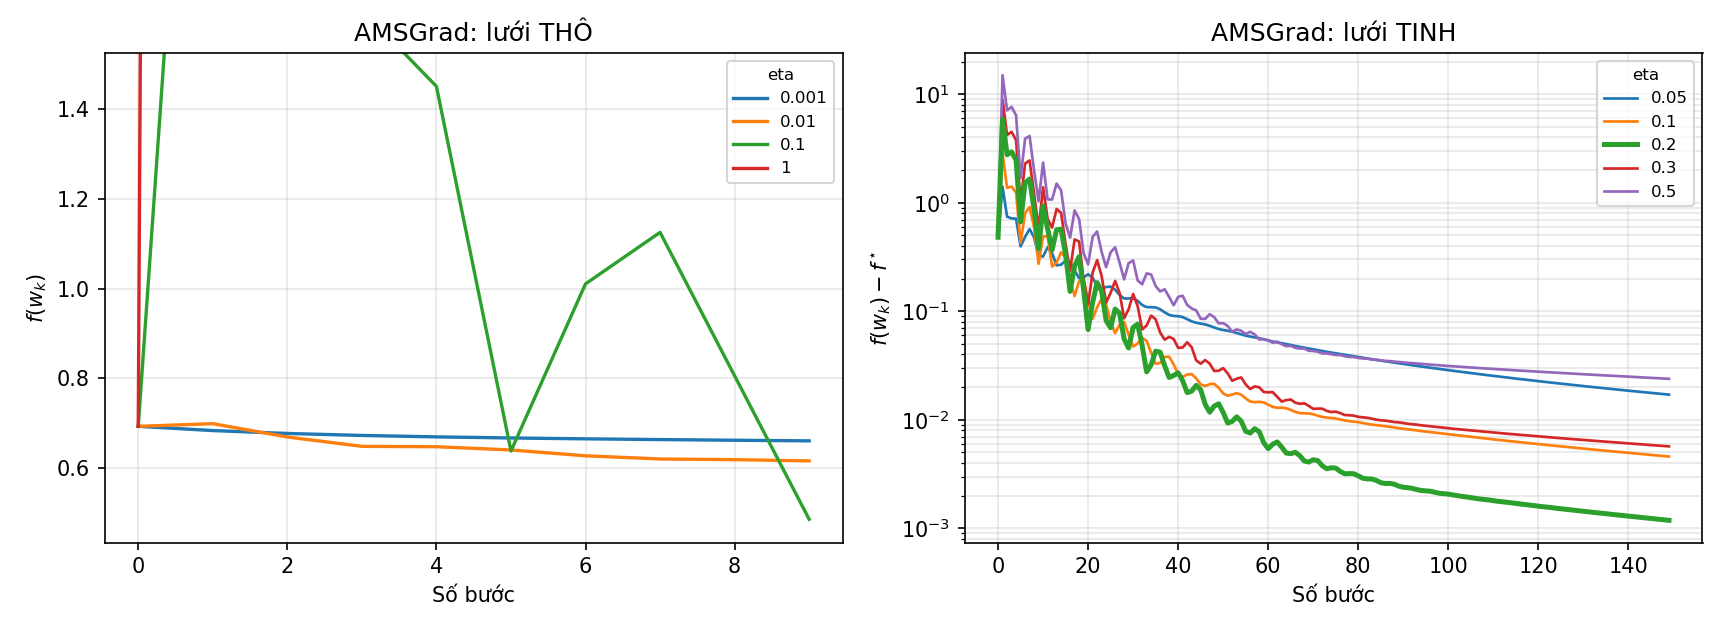
\includegraphics[width=0.94\linewidth]{tune_ada_amsgrad}}{}
  \end{center}
  \vspace{-2pt}
  {\scriptsize\nx{}}
  \begin{itemize}\scriptsize\itemsep=1pt
    \item Lưới thô (trục thẳng): $\eta=1$ vọt lên, $\eta\le0{,}01$ gần như đứng yên --- vùng cần dò
          nằm quanh $0{,}1$.
    \item Lưới tinh (thang log): $\eta=\mathbf{0{,}2}$ rõ ràng là cực tiểu \emph{nội} --- $0{,}1$ cho
          $4{,}6\!\cdot\!10^{-3}$ và $0{,}3$ cho $5{,}7\!\cdot\!10^{-3}$, đều tệ hơn.
    \item Bốn thuật toán còn lại có hình tương tự trong \texttt{artifacts/figures/tune\_ada\_*.png}.
  \end{itemize}
\end{frame}

\begin{frame}{6. MỘT SỐ THUẬT TOÁN TỐI ƯU KHÁC}{6.6. Kết quả: họ Ada/Adam so với GD, AGD, Newton}
  \begin{center}
    \IfFileExists{../artifacts/figures/adaptive_family_ridge.png}
      {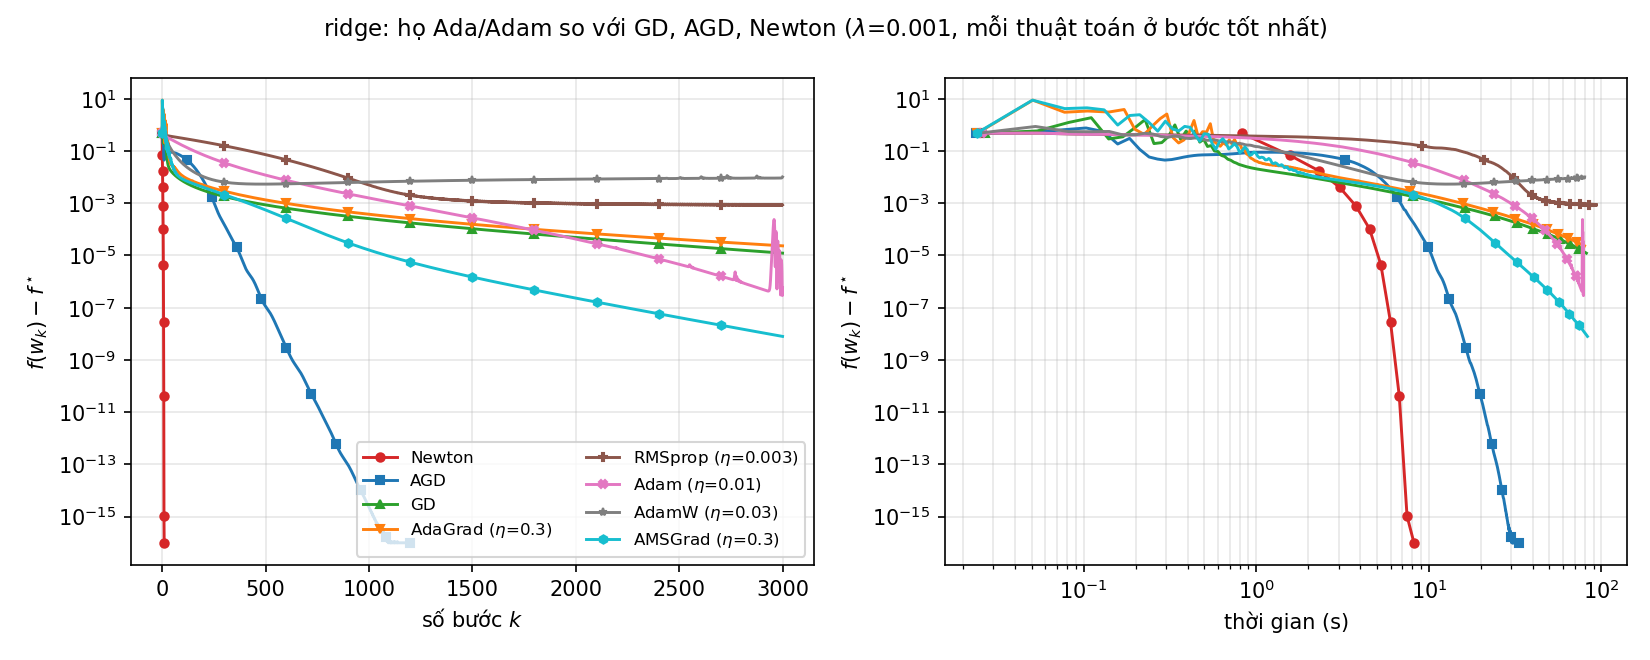
\includegraphics[width=0.90\linewidth]{adaptive_family_ridge}}{}
  \end{center}
  \vspace{-2pt}
  {\scriptsize\nx{} tám đường trên cùng một hàm mục tiêu, cùng điểm xuất phát, cùng trần
  \num{3000} bước; mỗi thuật toán thích nghi chạy ở $\eta$ tốt nhất của riêng nó và GD chạy ở bước
  dò tay $t=0{,}4$. \textbf{Chỉ AGD và Newton chạm tiêu chí dừng}; cả họ bước-thích-nghi đều nằm
  lại trên trần, còn AGD về đúng $f^\star$ sau \num{1202} vòng. Số liệu và thứ hạng ở mục 6.7.}
\end{frame}

\begin{frame}{6. MỘT SỐ THUẬT TOÁN TỐI ƯU KHÁC}{6.7. Họ Ada/Adam --- bảng số và thứ hạng}
  \begin{columns}[T]
    \begin{column}{0.36\textwidth}
      \begin{center}\scriptsize
      \begin{tabular}{lccc}
        \toprule
        & $\eta$ & Bước & $f-f^\star$\\
        \midrule
        Newton  & ---          & \textbf{10}  & $0$\\
        AGD     & ---          & \num{1202}   & $0$\\
        AMSGrad & \num{0.3}    & $\times$     & $\mathbf{8{,}0\!\cdot\!10^{-9}}$\\
        Adam    & \num{0.01}   & $\times$     & $5{,}7\!\cdot\!10^{-7}$\\
        \textbf{GD} & ---      & $\times$     & $\mathbf{1{,}2\!\cdot\!10^{-5}}$\\
        AdaGrad & \num{0.3}    & $\times$     & $2{,}3\!\cdot\!10^{-5}$\\
        RMSprop & \num{0.003}  & $\times$     & $8{,}7\!\cdot\!10^{-4}$\\
        AdamW$^\ddagger$ & \num{0.03} & $\times$ & $1{,}0\!\cdot\!10^{-2}$\\
        \bottomrule
      \end{tabular}
      \end{center}
    \end{column}
    \begin{column}{0.64\textwidth}\scriptsize
      \nx{} $\times$ $=$ chạm trần \num{3000} bước, chưa đạt tiêu chí dừng. GD và AGD chạy bước
      \textbf{dò tay} ($0{,}4$ và $0{,}3$) đúng như money plot. Cột $\eta$ ở đây \emph{khác} mục
      6.4--6.5 (AMSGrad $0{,}3$ so với $0{,}2$, Adam $0{,}01$ so với $0{,}12$) vì nó được quét lại
      ở \textbf{ngân sách \num{3000} vòng}, còn mục 6.4 dò ở 150 vòng --- chính hiện tượng mà 6.4
      đã cảnh báo: $\eta$ tốt nhất phụ thuộc ngân sách.
      \begin{itemize}\itemsep=2pt
        \item \textbf{Chỉ AGD và Newton hội tụ.} Không thuật toán bước-thích-nghi nào về đích, dù
              AMSGrad (tốt nhất trong họ) hơn GD hơn \textbf{3 bậc}.
        \item \textbf{Ba trong năm thuật toán thích nghi THUA GD thuần}: AdaGrad
              ($2{,}3\!\cdot\!10^{-5}$), RMSprop, AdamW đều tệ hơn $1{,}2\!\cdot\!10^{-5}$ của GD
              ở $t=0{,}4$. Chỉ Adam và AMSGrad vượt được. Cơ chế thích nghi \emph{không} miễn phí:
              nó đổi một bước dở lấy một bước trung bình, chứ không thay được việc dò bước tử tế.
        \item \textbf{ĐẢO CHIỀU so với bài toán nhỏ.} Ở $d=39$ Adam về đích sau 413 bước còn AGD
              cần 800; ở $d=415$, cùng đoạn code, AGD hội tụ sau \num{2400} bước còn Adam thì
              không. \emph{Đừng kết luận từ bài toán nhỏ}: khi $\kappa$ tăng, điều chỉnh theo
              đường chéo không thay được thông tin cong đầy đủ.
        \item $^\ddagger$AdamW: xem mục 6.8.
      \end{itemize}
    \end{column}
  \end{columns}
\end{frame}

\begin{frame}{6. MỘT SỐ THUẬT TOÁN TỐI ƯU KHÁC}{6.8. Hai biến thể của Adam --- số đo nói gì}
  \small
  \textbf{AMSGrad --- cơ chế ở mục 6.3 hoạt động đúng như hứa.}
  \begin{itemize}\footnotesize
    \item $8{,}0\times10^{-9}$ so với $5{,}7\times10^{-7}$ của Adam --- \textbf{tốt hơn 72 lần}, và
          là kết quả tốt nhất trong cả họ bước-thích-nghi.
    \item Mẫu số $\sqrt{\hat v_k}$ không giảm nên bước hiệu dụng đơn điệu không tăng. Đó đúng là
          tính chất RMSprop thiếu, và cũng là lý do RMSprop dừng ở sàn $8{,}7\times10^{-4}$.
          Công thức ở mục 6.3 giờ có số đo đi kèm.
  \end{itemize}
  \vspace{2pt}
  \textbf{AdamW --- $1{,}0\times10^{-2}$ KHÔNG có nghĩa là tối ưu kém.}
  \begin{itemize}\footnotesize
    \item Nó về đúng nghiệm của \emph{một bài toán khác} (mục 6.3). Hai bằng chứng đo được:
          sàn \textbf{không đổi} theo $\eta$ ($1{,}0$--$1{,}1\times10^{-2}$ với mọi
          $\eta\in[0{,}003;\,0{,}1]$) --- nếu là chuyện tối ưu thì $\eta$ phải ảnh hưởng; và
          khoảng cách còn \textbf{tăng} theo thời gian ($6{,}5\times10^{-3}$ ở bước \num{1000}
          $\to 1{,}0\times10^{-2}$ ở bước \num{3000}) --- một thuật toán tối ưu kém thì đứng yên,
          không đi xa dần.
    \item Bài học: khi so sánh thuật toán, phải kiểm tra chúng có cùng \emph{điểm dừng} không ---
          nếu không thì bảng xếp hạng đang so hai bài toán khác nhau.
  \end{itemize}
\end{frame}

% =====================================================================
\section{Mở rộng: bài toán Lasso}
% =====================================================================

\begin{frame}{7. MỞ RỘNG SANG BÀI TOÁN LASSO}{7.1. Bài toán và phương pháp Subgradient}
  \label{sec:7}%
  \small
  Với hàm phạt Lasso, hàm mục tiêu trở thành
  \[
    F(w)=\underbrace{\frac1n\sum_{i=1}^n\ell_i(w)}_{\text{trơn, lồi}}+\underbrace{\alpha\norm{w}_1}_{\text{lồi, \textbf{không trơn}}}
  \]
  Hàm vẫn lồi nhưng \textbf{không khả vi} tại mọi điểm có tọa độ bằng 0 $\Rightarrow$ không dùng
  được GD và Newton như cũ. Điều kiện tối ưu đổi từ $\nabla F=0$ thành $0\in\partial F(\wstar)$.
  \vspace{6pt}

  \textbf{Phương pháp Subgradient:} giống Gradient Descent nhưng thay gradient bằng subgradient
  \[
    w^{(k)}=w^{(k-1)}-t_k\,g^{(k-1)},\qquad g^{(k-1)}\in\partial F\big(w^{(k-1)}\big)
  \]
  với $\partial\norm{w}_1$ lấy $\mathrm{sign}(w_j)$ nếu $w_j\ne0$ và một giá trị bất kỳ trong $[-1,1]$ nếu $w_j=0$.
  \vspace{4pt}

  \nx{} tốc độ chỉ $O(1/\sqrt k)$, quỹ đạo không đơn điệu, và nghiệm \textbf{không thưa thật sự}
  (các hệ số chỉ tiến \emph{gần} 0 chứ không \emph{bằng} 0).
\end{frame}

\begin{frame}{7. MỞ RỘNG SANG BÀI TOÁN LASSO}{7.2. Dò $\eta_0$ cho subgradient}
  \begin{center}
    {\large\color{accent}\textbf{$\rightarrow$ Chọn $\eta_0 = 2$}}
  \end{center}
  \vspace{-6pt}
  \begin{center}
    \IfFileExists{../artifacts/figures/tune_l1_subgradient.png}
      {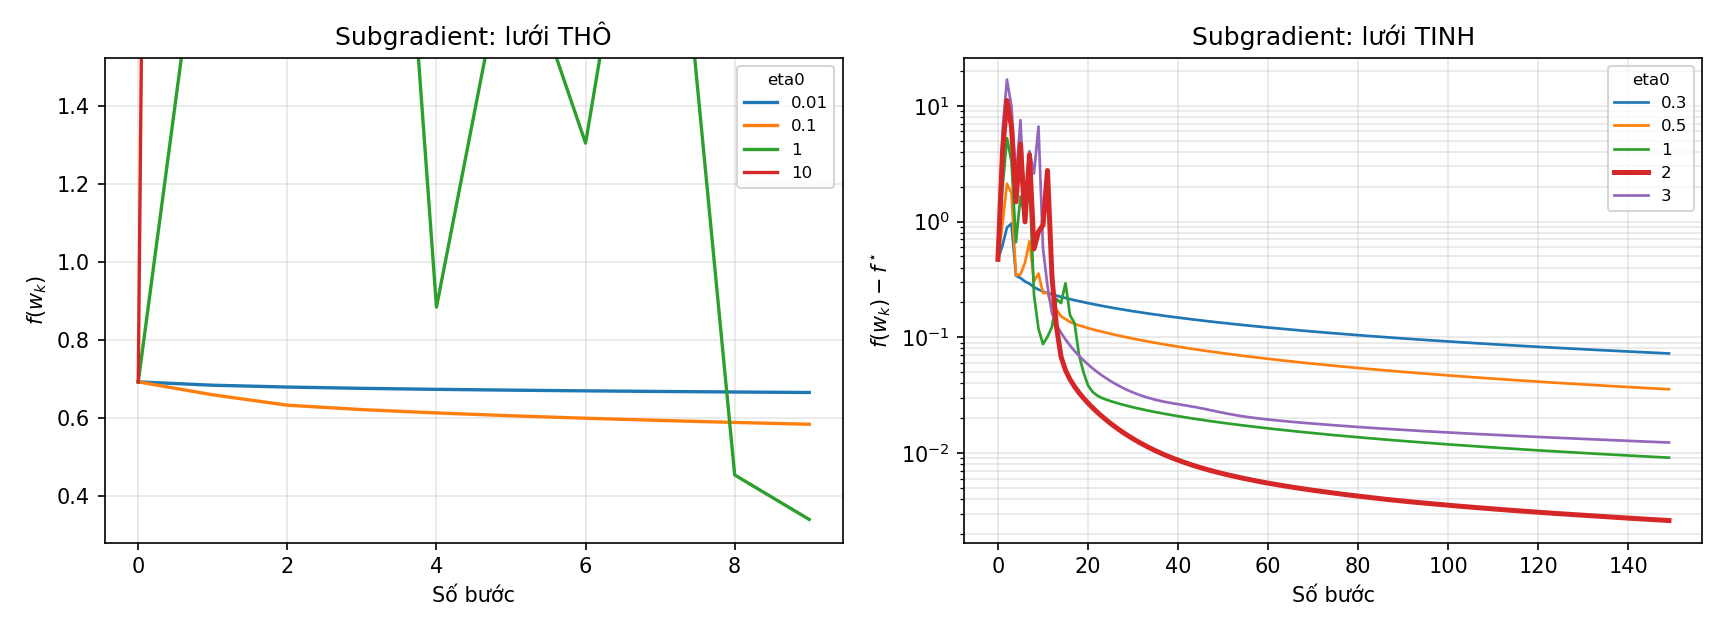
\includegraphics[width=0.94\linewidth]{tune_l1_subgradient}}{}
  \end{center}
  \vspace{-2pt}
  {\scriptsize\nx{}}
  \begin{itemize}\scriptsize\itemsep=1pt
    \item $\eta_0=\mathbf{2}$, cực tiểu nội: $1{,}0$ cho $9{,}1\!\cdot\!10^{-3}$, $3{,}0$ cho
          $1{,}2\!\cdot\!10^{-2}$, còn $2{,}0$ cho $2{,}6\!\cdot\!10^{-3}$.
    \item Dò $\eta_0$ cẩn thận là bắt buộc ở đây: một phương pháp subgradient trông tệ vì bị cho
          bước sai thì không chứng minh được điều gì về subgradient cả.
  \end{itemize}
\end{frame}

\begin{frame}{7. MỞ RỘNG SANG BÀI TOÁN LASSO}{7.3. Phương pháp Proximal Gradient Descent}
  \small
  Tách $F=f_0+h$ với $f_0$ trơn và $h=\alpha\norm{w}_1$. Mỗi bước làm một bước gradient trên $f_0$
  rồi chiếu qua toán tử prox của $h$:
  \[
    w^{(k)}=\prox_{t_k h}\Big(w^{(k-1)}-t_k\,\nabla f_0\big(w^{(k-1)}\big)\Big),
    \qquad
    \prox_{t\alpha\norm{\cdot}_1}(v)_j=\mathrm{sign}(v_j)\max\big(|v_j|-t\alpha,\,0\big)
  \]
  Toán tử này gọi là \textbf{soft-thresholding}: nó đặt các tọa độ \emph{đúng bằng} 0 $\Rightarrow$
  nghiệm thưa thật sự.
  \vspace{4pt}
  \begin{itemize}
    \item \textbf{Độ dài bước cố định} — tốc độ $O(1/k)$ (thuật toán ISTA);
    \item \textbf{Backtracking} — như GD nhưng kiểm tra trên toán tử gradient tổng quát $G_t(w)$;
    \item \textbf{Acceleration} — thêm động lượng Nesterov, tốc độ $O(1/k^2)$ (thuật toán
          FISTA~\cite{beck2009fista}).
  \end{itemize}
  \vspace{2pt}
  \nx{} đúng một mẹo động lượng biến GD thành AGD ($\kappa\to\sqrt\kappa$) cũng biến
  ISTA thành FISTA ($1/k\to1/k^2$) — gia tốc là một \emph{nguyên lý} chung.
\end{frame}

\begin{frame}{7. MỞ RỘNG SANG BÀI TOÁN LASSO}{7.4. Dò bước cho ISTA --- ba vòng mới tới}
  \begin{center}
    {\large\color{accent}\textbf{$\rightarrow$ Chọn $t = 7/L$}}
  \end{center}
  \vspace{-6pt}
  \begin{center}
    \IfFileExists{../artifacts/figures/tune_l1_ista.png}
      {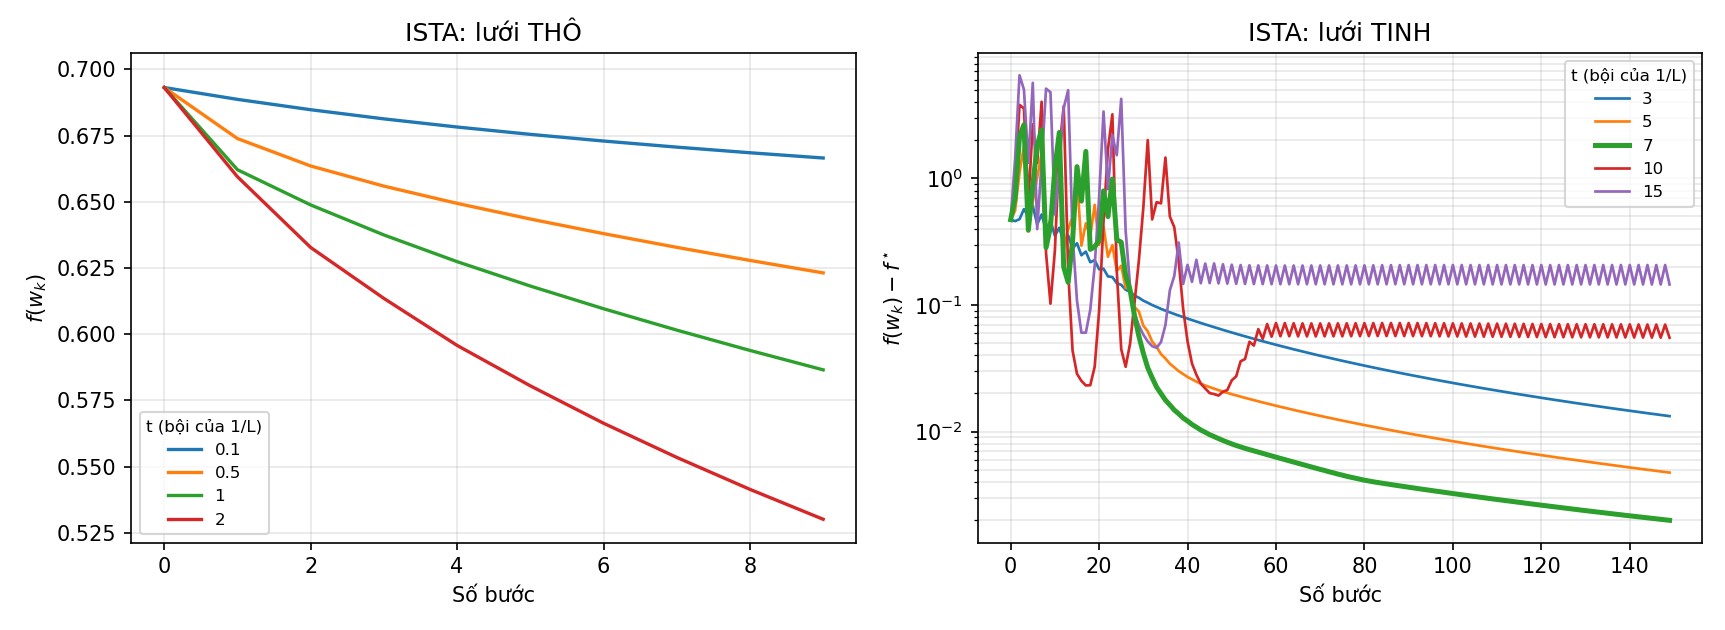
\includegraphics[width=0.74\linewidth]{tune_l1_ista}}{}
  \end{center}
  \vspace{-2pt}
  {\scriptsize\nx{}}
  \begin{itemize}\scriptsize\itemsep=1pt
    \item Phải dò \textbf{ba vòng}: cả $2{,}5/L$ lẫn $7/L$ đều chạm mép trên, tới vòng thứ ba mới
          thấy $10/L$ hỏng hẳn và $\mathbf{7/L}$ là cực tiểu nội.
    \item Lý thuyết proximal đòi $t\le 1/L$. Bước tốt nhất là $7/L$ --- \textbf{cận bi quan gấp 7
          lần}, đúng kiểu đã gặp ở GD (mục 4.7, bước $0{,}4$ so với ngưỡng $2/L=0{,}142$).
    \item Điểm chung cả bài: các cận $1/L$, $2/L$ là \emph{đủ} để có bảo đảm, không \emph{cần} để
          chạy tốt. Nhưng \textbf{đừng đem $7/L$ này sang FISTA} --- mục 7.5.
  \end{itemize}
\end{frame}

\begin{frame}{7. MỞ RỘNG SANG BÀI TOÁN LASSO}{7.5. Dò bước cho FISTA --- vì sao không dùng lại $7/L$ của ISTA}
  \begin{center}
    {\large\color{accent}\textbf{$\rightarrow$ Chọn $t = 4/L$}}
  \end{center}
  \vspace{-6pt}
  \begin{center}
    \IfFileExists{../artifacts/figures/tune_l1_fista.png}
      {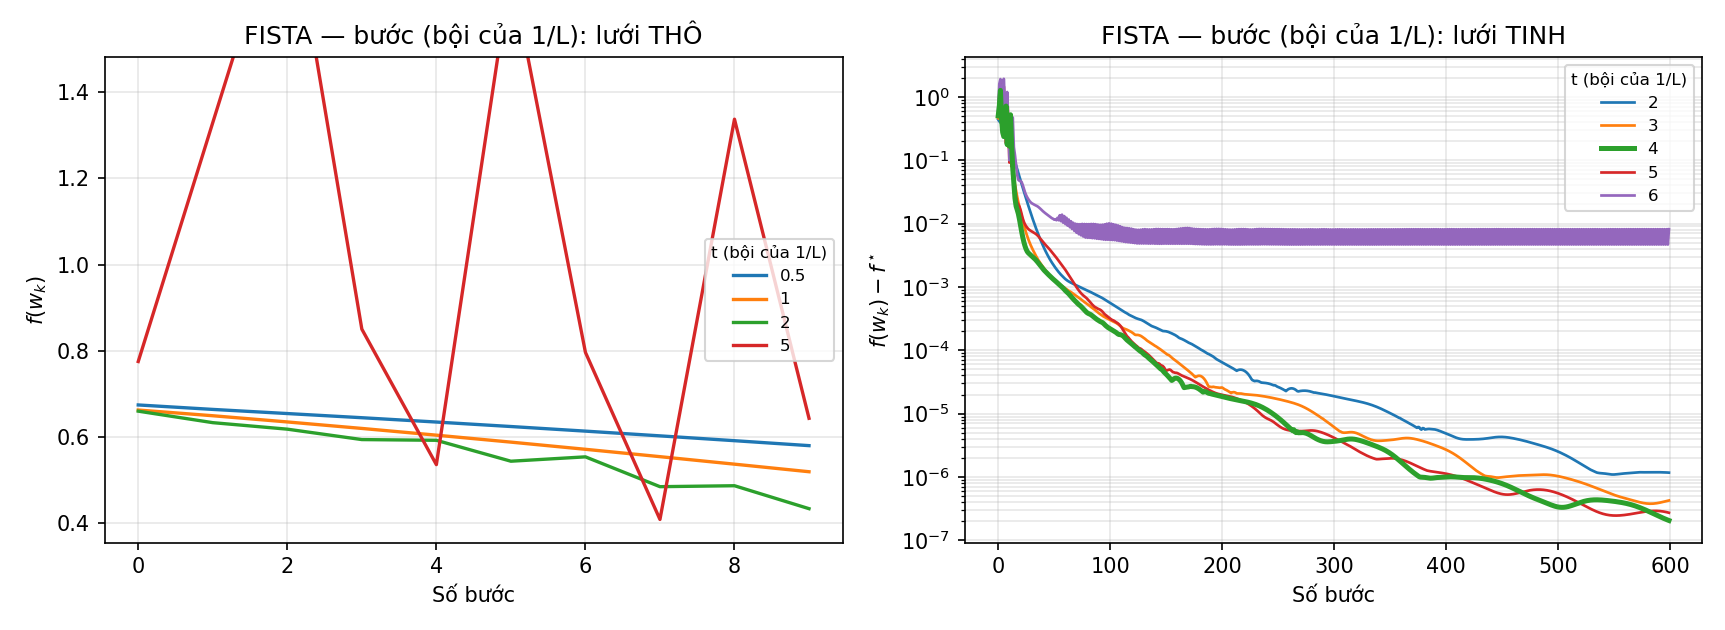
\includegraphics[width=0.68\linewidth]{tune_l1_fista}}{}
  \end{center}
  \vspace{-2pt}
  {\scriptsize\nx{} lưới tinh 600 vòng: $2\to\num{1.17e-6}$, $3\to\num{4.26e-7}$,
  $\mathbf{4\to\num{2.06e-7}}$, $5\to\num{2.72e-7}$, rồi $6$ \textbf{sập} xuống $\num{8.15e-3}$
  --- và cùng lúc số hệ số khác $0$ vọt từ $125$ lên $346$, tức nghiệm mất luôn tính thưa.}
  \begin{itemize}\scriptsize\itemsep=1pt
    \item \textbf{Trần bước của FISTA thấp hơn của ISTA}: vách sập nằm giữa $5/L$ và $6/L$, trong
          khi ISTA vẫn chạy tốt ở $7/L$. Bản \emph{gia tốc} chịu bước ngắn hơn bản thường.
    \item Cùng cơ chế với mục 4.12: momentum \textbf{tích lũy} phần vượt ngưỡng qua các vòng, còn
          ISTA thuần thì mỗi bước tự hấp thụ. Gia tốc mua tốc độ bằng \emph{biên an toàn}.
    \item Bài học quy trình: \textbf{tham số dò cho thuật toán nào chỉ dùng cho thuật toán đó}.
          Thử dùng lại $7/L$ cho FISTA cho $\num{1.17e-2}$ --- tệ hơn cả bước $1/L$ theo sách.
  \end{itemize}
\end{frame}

\begin{frame}{7. MỞ RỘNG SANG BÀI TOÁN LASSO}{7.6. Kết quả trên bộ dữ liệu \texttt{lasso} ($d=519$)}
  \begin{center}
    \IfFileExists{../artifacts/figures/l1_lasso.png}
      {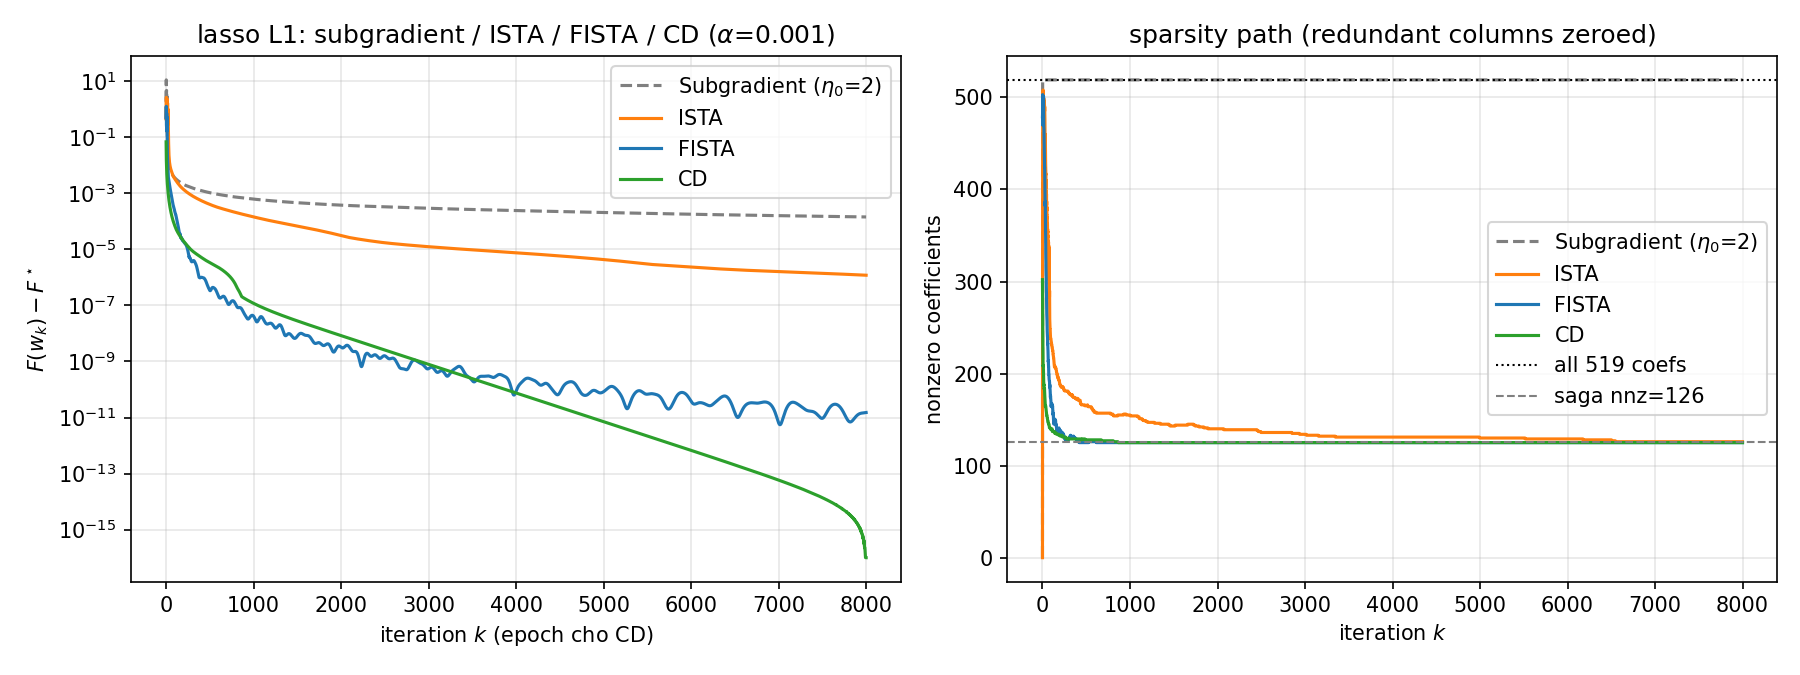
\includegraphics[width=0.94\linewidth]{l1_lasso}}{}
  \end{center}
  \vspace{-2pt}
  {\scriptsize\nx{} bốn phương pháp, mỗi cái ở bước \textbf{dò tay} của riêng nó (mục 7.2, 7.4,
  7.5). Thứ tự về đích đúng như tốc độ lý thuyết $O(1/\sqrt k)<O(1/k)<O(1/k^2)$: subgradient
  $\num{1.4e-4}$, ISTA $\num{1.2e-6}$, FISTA $\num{1.5e-11}$, còn \textbf{CD} --- solver
  \texttt{scikit-learn} thực dùng cho Lasso~\cite{friedman2010glmnet} --- về đúng $f^\star$. Bảng số
  và chuyện tính thưa ở mục 7.7.}
\end{frame}

\begin{frame}{7. MỞ RỘNG SANG BÀI TOÁN LASSO}{7.7. Lasso --- số bước, độ chính xác và tính thưa}
  \begin{columns}[T]
    \begin{column}{0.44\textwidth}\scriptsize
      \begin{center}\scriptsize
      \begin{tabular}{lccc}
        \toprule
        Thuật toán & Tốc độ LT & Số bước & Hệ số $\ne0$\\
        \midrule
        Subgradient & $O(1/\sqrt k)$ & \num{8000}$^\dagger$ & \textbf{\num{519}}\\
        ISTA  & $O(1/k)$   & \num{8000}$^\dagger$ & \num{126}\\
        FISTA & $O(1/k^2)$ & \num{8000}$^\dagger$ & \num{125}\\
        CD    & (thực tế nhanh) & \num{8000}$^\dagger$ & \num{125}\\
        \texttt{saga} & --- & \num{5000} & \num{126}\\
        \bottomrule
      \end{tabular}
      \end{center}
      {\tiny $^\dagger$ chạm trần \num{8000} vòng. Mỗi thuật toán ở bước \textbf{đã dò tay}:
      subgradient $\eta_0{=}2$ (7.2), ISTA $7/L$ (7.4), FISTA $4/L$ (7.5).
      $f-f^\star$ cuối: subgradient $1{,}4\!\cdot\!10^{-4}$, ISTA $1{,}2\!\cdot\!10^{-6}$,
      FISTA $1{,}5\!\cdot\!10^{-11}$, \textbf{CD $0$}, \texttt{saga} $7{,}1\!\cdot\!10^{-7}$.}
    \end{column}
    \begin{column}{0.56\textwidth}\scriptsize
      \nx{}
      \begin{itemize}\scriptsize\itemsep=2pt
        \item \textbf{Subgradient để lại đủ \num{519}/\num{519} hệ số khác 0} --- không thưa
              \emph{chút nào}; prox đưa xuống \num{125}. Nó cũng chậm nhất, và thứ tự
              $O(1/\sqrt k)<O(1/k)<O(1/k^2)$ hiện ra đúng \emph{dù mỗi thuật toán đã được cho
              bước tốt nhất của riêng nó}: $\num{1.4e-4}$, $\num{1.2e-6}$, $\num{1.5e-11}$ ---
              cách nhau đều đặn $\sim$2 và $\sim$5 bậc.
        \item $\operatorname{sign}(w)=\pm1$ ở \emph{mọi} tọa độ khác 0 nên subgradient đẩy tọa độ
              \emph{qua} $0$ rồi đổi dấu, không bao giờ đáp đúng vào $0$. Soft-thresholding không
              phải cách nhanh hơn để làm cùng việc --- nó \emph{là} phần tạo ra tính thưa.
        \item \textbf{CD} thắng tất cả (đạt đúng $f^\star$) và là solver \texttt{scikit-learn} thực
              dùng cho Lasso~\cite{friedman2010glmnet}. Bốn cài đặt độc lập --- ISTA, FISTA, CD,
              \texttt{saga} --- cùng cho \textbf{125--126/\num{519}}: L1 loại $\sim$76\% cột.
              Việc dò bước cũng sửa luôn ISTA: ở $1/L$ nó còn để lại \num{148} hệ số, ở $7/L$ thì
              về \num{126} --- \emph{cùng} tập thưa với ba phương pháp kia.
      \end{itemize}
    \end{column}
  \end{columns}
\end{frame}

% =====================================================================
\section{Kết luận}
% =====================================================================

\begin{frame}{8. KẾT LUẬN}{8.1. Về dữ liệu và về từng thuật toán}
  \label{sec:8}%
  \footnotesize
  \begin{itemize}\itemsep=1pt
    \item \textbf{Chuẩn hóa không phải mẹo tinh chỉnh mà là điều kiện để chạy được.} Ở $d=415$,
          bộ thô có $\kappa\approx10^{19}$ --- vượt dải số thực 64 bit --- nên $\lambda I$ thành vô
          hình, Hessian suy biến về mặt số học và \textbf{Newton không chạy nổi}; GD/AGD sau
          \num{2000} bước còn cách nghiệm $0{,}434$ (mục 4.1).
    \item Thực nghiệm khẳng định $\kappa$ vs $\sqrt\kappa$: độ dốc log--log đo được là
          \num{0.819} (GD) và \num{0.413} (AGD), \textbf{tỉ số $1{,}98\approx2$}. Cả hai dưới giá
          trị lý thuyết vì $\kappa\log\frac1\epsilon$ là \emph{cận trên} (mục 5.5).
    \item \textbf{Backtracking giúp GD nhưng phá AGD} (vòng chạy riêng, trần \num{5000} bước): GD
          đi từ $3{,}3\times10^{-4}$ xuống $7{,}8\times10^{-8}$ --- hơn \textbf{4 bậc}; còn AGD từ
          hội tụ sau \num{2131} bước thành \emph{không} hội tụ. Đổi bước mỗi vòng là phá cặp
          $(t,\beta)$; đổi $t$ mà \emph{tính lại} $\beta$ thì không sao --- đó là cấu hình AGD ở
          mục 4.17, nhanh hơn bản $1/L$ 2,0 lần.
    \item \textbf{Newton nhanh nhất trong bảy cấu hình của nhóm, trên \emph{cả hai} trục}: 8--10
          bước so với hàng nghìn, và \num{6.0}s so với \num{11.4}--\num{583.2}s (mục 4.18). Nhưng
          nó \textbf{thua quasi-Newton của thư viện}: chi phí $O(nd^2+d^3)$ đủ nặng để
          \texttt{lbfgs} về trước (\num{3.31}s so với \num{10.21}s, mục 4.19) --- đúng điểm hòa vốn
          dự báo ($d^\star\approx139$).
    \item \textbf{Cài đặt:} giải hệ bằng Cholesky, không nghịch đảo Hessian. Ma trận phải
          \textbf{đủ hạng} --- ở $d\sim400$ điều đó không tự nhiên mà có: corr/VIF không bắt được
          cộng tuyến \emph{chính xác}, phải thêm QR xoay cột.
    \item \textbf{SGD} đạt $1{,}6\times10^{-3}$ sau 50 epoch rồi dừng ở sàn phương sai.
  \end{itemize}
\end{frame}

\begin{frame}{8. KẾT LUẬN}{8.2. Về các phần mở rộng và về độ tin cậy của cài đặt}
  \footnotesize
  \begin{itemize}\itemsep=1pt
    \item Họ \textbf{bước thích nghi} \emph{không} thắng nổi GD một khi GD được dò bước tử tế:
          chỉ Adam ($1{,}3$ bậc) và AMSGrad ($3{,}2$ bậc) vượt lên, còn AdaGrad, RMSprop, AdamW
          đều \textbf{thua} GD ở $t=0{,}4$ (mục 6.7). Và không cái nào thắng AGD --- ở $d=415$ chỉ
          AGD và Newton đạt tiêu chí dừng. Đáng chú ý, ở $d=39$ Adam từng \emph{thắng} AGD (413 so
          với 800 bước): cùng đoạn code, bài toán lớn hơn thì kết luận \textbf{đảo chiều}.
    \item Với bài toán \textbf{không khả vi} (Lasso), nhóm đã chạy \emph{cả} subgradient để đối
          chứng: nó để lại \textbf{\num{519}/\num{519}} hệ số khác 0 trong khi proximal đưa xuống
          \num{125}, và còn chậm hơn cả ISTA. Soft-thresholding không phải cách nhanh hơn để làm
          cùng một việc --- nó \emph{là} phần tạo ra tính thưa.
    \item Cùng \textbf{mẹo động lượng} biến GD thành AGD ($\kappa\to\sqrt\kappa$) cũng biến ISTA
          thành FISTA ($1/k\to1/k^2$): gia tốc là một \emph{nguyên lý} chung.
    \item Kết quả code nhóm tự cài \textbf{khớp với thư viện} \texttt{scikit-learn} tới độ chính xác
          máy ($\lvert f-f^\star\rvert\sim10^{-17}$), và ba cài đặt L1 độc lập (FISTA, CD,
          \texttt{saga}) cùng hội tụ về \textbf{125--126 / 519} hệ số khác 0 --- hai phép kiểm tra
          chéo độc lập cho thấy cài đặt là đúng.
    \item $f^\star$ kèm \textbf{chứng chỉ} chứ không đòi tin: $\norm{\nabla f(\wstar)}=\num{7.9e-15}$
          và tính lồi mạnh cho $f^\star-f_{\text{true}}\le\num{3.1e-26}$ (mục 4.2, Phụ lục B).
  \end{itemize}
\end{frame}

% ----------------------------------------------------------- Tài liệu
\begin{frame}[allowframebreaks]{Tài liệu tham khảo}
    \printbibliography[heading=none]
\end{frame}

% =====================================================================
% PHỤ LỤC
% =====================================================================
\appendix

\begin{frame}[plain]
  \begin{center}{\Large\color{accent}\textbf{Phụ lục}}\end{center}
\end{frame}

\begin{frame}[fragile]{Phụ lục A}{Cài đặt lõi và kiểm chứng đạo hàm}
\begin{lstlisting}
# reg[j] = 1, RIENG reg[-1] = 0: he so chan KHONG bi phat (muc 5.1)
def value(w, X, y, lam, reg):          # on dinh so: dung logaddexp
    z = X @ w
    return np.mean(np.logaddexp(0.0, z) - y*z) + 0.5*lam*np.sum((reg*w)**2)

def grad(w, X, y, lam, reg):
    p = sigmoid(X @ w)
    return X.T @ (p - y) / len(y) + lam*reg*w

def hessian(w, X, y, lam, reg):        # Newton = IRLS
    p = sigmoid(X @ w); s = p*(1-p)
    H = (X.T * s) @ X / len(y)
    H[np.diag_indices(len(w))] += lam*reg
    return H
\end{lstlisting}
  \footnotesize
  \begin{itemize}
    \item Kiểm chứng: \texttt{scipy.optimize.check\_grad} cho sai số $\approx10^{-7}$;
          Hessian đối chiếu bằng sai phân trung tâm, khớp $\sim10^{-7}$.
    \item Newton dùng \texttt{cholesky} $+$ \texttt{solve}, không dùng \texttt{inv}.
    \item \texttt{reg} không phải chi tiết vụn: chính số $0$ ở hệ số chặn làm $\mu\ne\lambda$, và
          là lý do mục 4.2 phải \emph{đo} $\mu^\star$ thay vì thay $\lambda$ vào.
  \end{itemize}
\end{frame}

\begin{frame}{Phụ lục B}{Giao thức đo và chỉ số phân loại}
  \small
  \textbf{Giao thức đo:}
  \begin{itemize}
    \item Khởi tạo chung $w_0=0$; dừng khi $\norm{\nabla f}_2\le10^{-10}$ hoặc chạm trần số bước.
          Bảng 4.19 dùng trần chặt hơn ($10^{-11}$; $10^{-12}$ cho Newton), nên số vòng ở đó
          lớn hơn ở mục 4.17.
    \item $f^\star$ là giá trị \textbf{tại điểm cuối} của Newton damped chạy sâu
          ($\norm{\nabla f}_2<10^{-14}$, mục 4.2), \emph{không} lấy $\min$ cả lịch sử. Bảo chứng là bất đẳng thức
          $f(w)-f^\star\le\norm{\nabla f(w)}^2/(2\mu_\star)$ với $\mu_\star=\lambda_{\min}(\nabla^2f(\wstar))
          =\num{1.00e-3}$ \emph{đo tại nghiệm} (không phải $\lambda$ theo nguyên tắc --- mục 5.1).
          Đo được: $\norm{\nabla f(\wstar)}=\num{7.9e-15}$ cho cận $\num{3.1e-26}$, tức thấp hơn
          sàn $10^{-16}$ của mọi đồ thị \textbf{mười bậc}.
    \item Bài L1 không lồi mạnh $\Rightarrow$ không có cận trên; ở đó $f^\star$ là giá trị nhỏ nhất mà
          \emph{mọi} lần chạy đạt được --- hướng an toàn, chỉ làm khoảng cách báo cáo lớn hơn.
    \item AGD ghi $f(w_k)$ cùng $\norm{\nabla f(y_{k-1})}$ --- cùng hàng, cùng điểm: bổ đề giảm với
          bước $1/L$ cho $f(w_k)\le f(y_{k-1})$, nên tiêu chí dừng chứng nhận đúng đại lượng được vẽ.
    \item Thời gian: \texttt{perf\_counter}, làm nóng 1 vòng, trung vị 3--5 lần. BLAS ghim 1 luồng và
          được \textbf{kiểm tra lại} qua \texttt{threadpoolctl} lúc chạy.
    \item Môi trường: Apple M1, 1 luồng BLAS; Python 3.12, numpy 1.26, scikit-learn 1.5.
  \end{itemize}
\end{frame}

\begin{frame}{Phụ lục C}{Chỉ số phân loại (ngoài trọng tâm)}
  \small
  \textbf{Chỉ số phân loại} (\emph{in-sample}, trên toàn bộ $n=\num{75026}$ dòng — chỉ để tham khảo,
  không phải trọng tâm của bài; pipeline không chia train/test vì đây là bài toán tối ưu):
  \begin{center}\footnotesize
  \begin{tabular}{lccccc}
    \toprule
    & Tỉ lệ rời bỏ & AUC & Accuracy & F1 & Precision/Recall\\
    \midrule
    \texttt{ridge} & $10{,}8\%$ & \num{0.910} & \num{0.912} & \num{0.494} & \num{0.647}/\num{0.399}\\
    \bottomrule
  \end{tabular}
  \end{center}
\end{frame}

\begin{frame}[plain]
    \begin{center}
      {\Large\color{accent}\textbf{CẢM ƠN THẦY VÀ CÁC BẠN ĐÃ LẮNG NGHE}}
    \end{center}
\end{frame}

\end{document}
